%%%%%%%%%%%%%%%%%%%%%%%%%%%%%%%%%%%%%%%%
%%%%%%%%%% initial setup %%%%%%%%%%%%%%%
%%%%%%%%%%%%% packages %%%%%%%%%%%%%%%%%
%%%%%%%%%%%%%%%%%%%%%%%%%%%%%%%%%%%%%%%%


%%%%%%%%%%%%%%%%%%%%%%%%%%%%%%%%%%%%%%%                                       
%   USE .EPS PICTURES AND FIGURES !!! %
%   ADD LIST OF SYMBOLLS !!!          %
%   ADD FIG OF THE HYPOTHESES (see ex1)    
%%%%%%%%%%%%%%%%%%%%%%%%%%%%%%%%%%%%%%%


% PAGE
\documentclass[12pt,a4paper]{article}
\usepackage[a4paper]{geometry} % margins 
\geometry{paper = a4paper,
  twoside=true, % don't put twoside=false here
  left=2.5cm,
  right=2.5cm,
  top= 2.5cm, %86.55685pt
  bottom=2cm,
  headsep=0.5cm,
  headheight= 1.5cm, %84.29048pt,
  footskip=0.8cm, %14.49998pt,
  heightrounded=false,
  includehead=false,
  includefoot=false,
  includeheadfoot=false,
  includemp=false,
  nomarginpar,
}
\usepackage{setspace} % to set space between lines
\usepackage{indentfirst}
\linespread{1.5}
\usepackage[utf8]{inputenc} % So it's quite necessary, whenever you use unicode (non ASCII) characters, to use the inputenc package, in order to have a meaningful output (or sometimes to make a successful run of (La)TeX)

% WU Formatting Notes from English Business Institute
%Spacing [Zeilenabstand] 
%     o Running text: 1.5 spaced [1,5 zeilig] 
%     o Footnotes, bibliography and block quotations: single‐spaced [einfach]. 
%Font and font sizes 
%     o The same highly legible typeface must be used throughout the thesis. Standard fonts are Calibri, Palatino or Times New Roman. 
%     o Colour can only be used for charts and other illustrations, never for text. 
%     o Section headings: 14 pt and bold. 
%     o Subsection headings: 12 pt and bold. 
%     o Running text: 12 pt. 
%     o Footnotes, headings of figures, charts, graphs, tables, etc.: 10 pt. 
%Margins [Seitenränder] 
%     o The standard setting for margins in Word is “Normal” (Top: 2.5cm, Bottom: 2cm, Left: 2.5cm, Right: 2.5cm). 
%     o Except for page numbers, nothing must be written in the margins (do not use “headers” and “footers”). 

% DATE AND TIME
\usepackage[useregional=numeric]{datetime2}


% LANDSCAPE PAGES
\usepackage{lscape} %landscape page


% LANGUAGE
%\usepackage[bulgarian]{babel} 
\usepackage[english]{babel} % it must be loaded before the "glossaries" usepackage for acronyms
%\usepackage[german]{babel}


% LOREUM IPSUM
\usepackage{blindtext}


% FONT
\usepackage[T1]{fontenc} % font 
\usepackage{mathptmx} % type of font here: Times = mathptmx
\usepackage{lmodern} %to use modern fonts; some people say that the package is old


% TABLE OF CONTENT
\usepackage[nottoc]{tocbibind}


% GRAPHS & ILLUSTRATIONS
\usepackage{graphicx} % illustrations
\usepackage{subcaption} % illustrations next to eachother
\usepackage{capt-of} % caption outside floats ???
\usepackage{pgfgantt} % project timeline with gantt
\usepackage{float} % put images next to each other
%\usepackage[inkscapeformat=eps]{svg} % to insert SVG pictures from Inkscape 
\usepackage{svg} % sensitive to small and large letters in the .svg file name!, "Event01" is not equal to "event01"

% ILLUSTRATION OF THESIS STRUCTURE
%\usetikzlibrary{positioning,fit,calc} %structure thesis
%\tikzstyle{block} = [draw=none, thick, minimum height=1cm, align=center, fill=blue!50]   %structure thesis
%\tikzstyle{arrow} = [thick,->,>=stealth] %structure thesis


% EXTERNAL LINKS
\usepackage{hyperref} % hyperlink
\usepackage{url} % hyperlink


% EXTERNAL PDFs
\usepackage{pdflscape} % adding a pdf to the document
\usepackage{pdfpages} %insert PDF files


% WATERMARK
%\usepackage[printwatermark]{xwatermark} % watermark
%\usepackage{tikz} % watermark %structure thesis
%\newsavebox\mybox % watermark
%\savebox\mybox{\tikz[color=gray,opacity=0.3]\node{ILIEVA};} % watermark
%\newwatermark*[ % watermark
%  allpages, % watermark
%  angle=45, % watermark
%  scale=8, % watermark
%  xpos=-50, % watermark
%  ypos=50 % watermark
%  ]{\usebox\mybox} % watermark
%\usepackage{lastpage}


% HEADER AND FOOTER
\usepackage{fancyhdr} % page number
\pagestyle{fancy} % in order to overtake the fancy-package style
\fancyhead{}
\fancyhead[R]{\leftmark} % header with the name of the selection on the right side
%\fancyhead[L]{\leftmark} % header with the name of the selection on the left side


% PAGE NUMBER
\fancyfoot{}
\fancyhf[OFR]{\thepage} % Odd + Footer + Right 
\fancyhf[EFL]{\thepage} % Even + Footer + Left  
%\rfoot{\thepage} % page number right
%lfoot{\thepage} % page number left
\pagenumbering{roman} % insert roman numbers


% REFERENCES
\usepackage{natbib} % references
\usepackage{citeref} % to add pages to citations


% APPENDIX
\usepackage{appendix} %appendix


% TABLES
\usepackage{longtable} %tables long
\usepackage{multirow}
%\usepackage{makecell} %for thinner/thicker lines; for a diagonal line in a cell 
\usepackage{booktabs}


% ACRONYMS
\usepackage[acronym]{glossaries}
\makeglossaries

\usepackage{etoolbox} % to control spacing, alignment, etc. in the glossary

\newglossarystyle{twocolumnleft}{%
  % base it on the list style
  \setglossarystyle{list}%
  % customize the glossary environment (the whole list)
  \renewenvironment{theglossary}%
    {\begin{description}}% Use description list
    {\end{description}}%
  % customize each glossary entry
  \renewcommand*{\glossaryentryfield}[5]{%
    \item[\makebox[4cm][l]{##1}]% acronym, fixed width box, left aligned
    \makebox[\dimexpr\linewidth-4cm-1em][l]{##2}% definition in next column
  }%
}

%DEFINE ACRONYMS
\newacronym{ai}{AI}{Artificial Intelligence}
\newacronym{bhar}{BHAR}{buy-hold abnormal returns}
\newacronym{car}{CAR}{cumulative abnormal returns}
\newacronym{caar}{CAAR}{cumulative average abnormal returns}
\newacronym{did}{DID}{Difference-in-difference}
\newacronym{EU}{EU}{European Union}
\newacronym{ebit}{EBIT}{Earnings before interest and tax}
\newacronym{gics}{GICS}{Global Industry Classification Standard}
\newacronym{nse}{NSE}{National Stock Exchange}
\newacronym{tse}{TSE}{Teheran Stock Exchange}

% CODE FORMATTING
\usepackage{listings}
\usepackage{xcolor}
\definecolor{codegreen}{rgb}{0,0.6,0}
\definecolor{codegray}{rgb}{0.5,0.5,0.5}
\definecolor{codepurple}{rgb}{0.58,0,0.82}
\definecolor{backcolour}{rgb}{0.95,0.95,0.92}

\lstdefinestyle{mystyle}{
    backgroundcolor=\color{backcolour},   
    commentstyle=\color{codegreen},
    keywordstyle=\color{magenta},
    numberstyle=\tiny\color{codegray},
    stringstyle=\color{codepurple},
    basicstyle=\ttfamily\footnotesize,
    breakatwhitespace=false,         
    breaklines=true,                 
    captionpos=b,                    
    keepspaces=true,                 
    numbers=left,                    
    numbersep=5pt,                  
    showspaces=false,                
    showstringspaces=false,
    showtabs=false,                  
    tabsize=2
}
\lstset{style=mystyle}



%%%%%%%%%%%%%%%%%%%%%%%%%%%%%%%%%%%%%%%%%%%%%%%%%%%%
%%%%%%%%% beginning of the document %%%%%%%%%%%%%%%%
%%%%%%%%%%%%%%%%%%%%%%%%%%%%%%%%%%%%%%%%%%%%%%%%%%%%
\begin{document}
\
%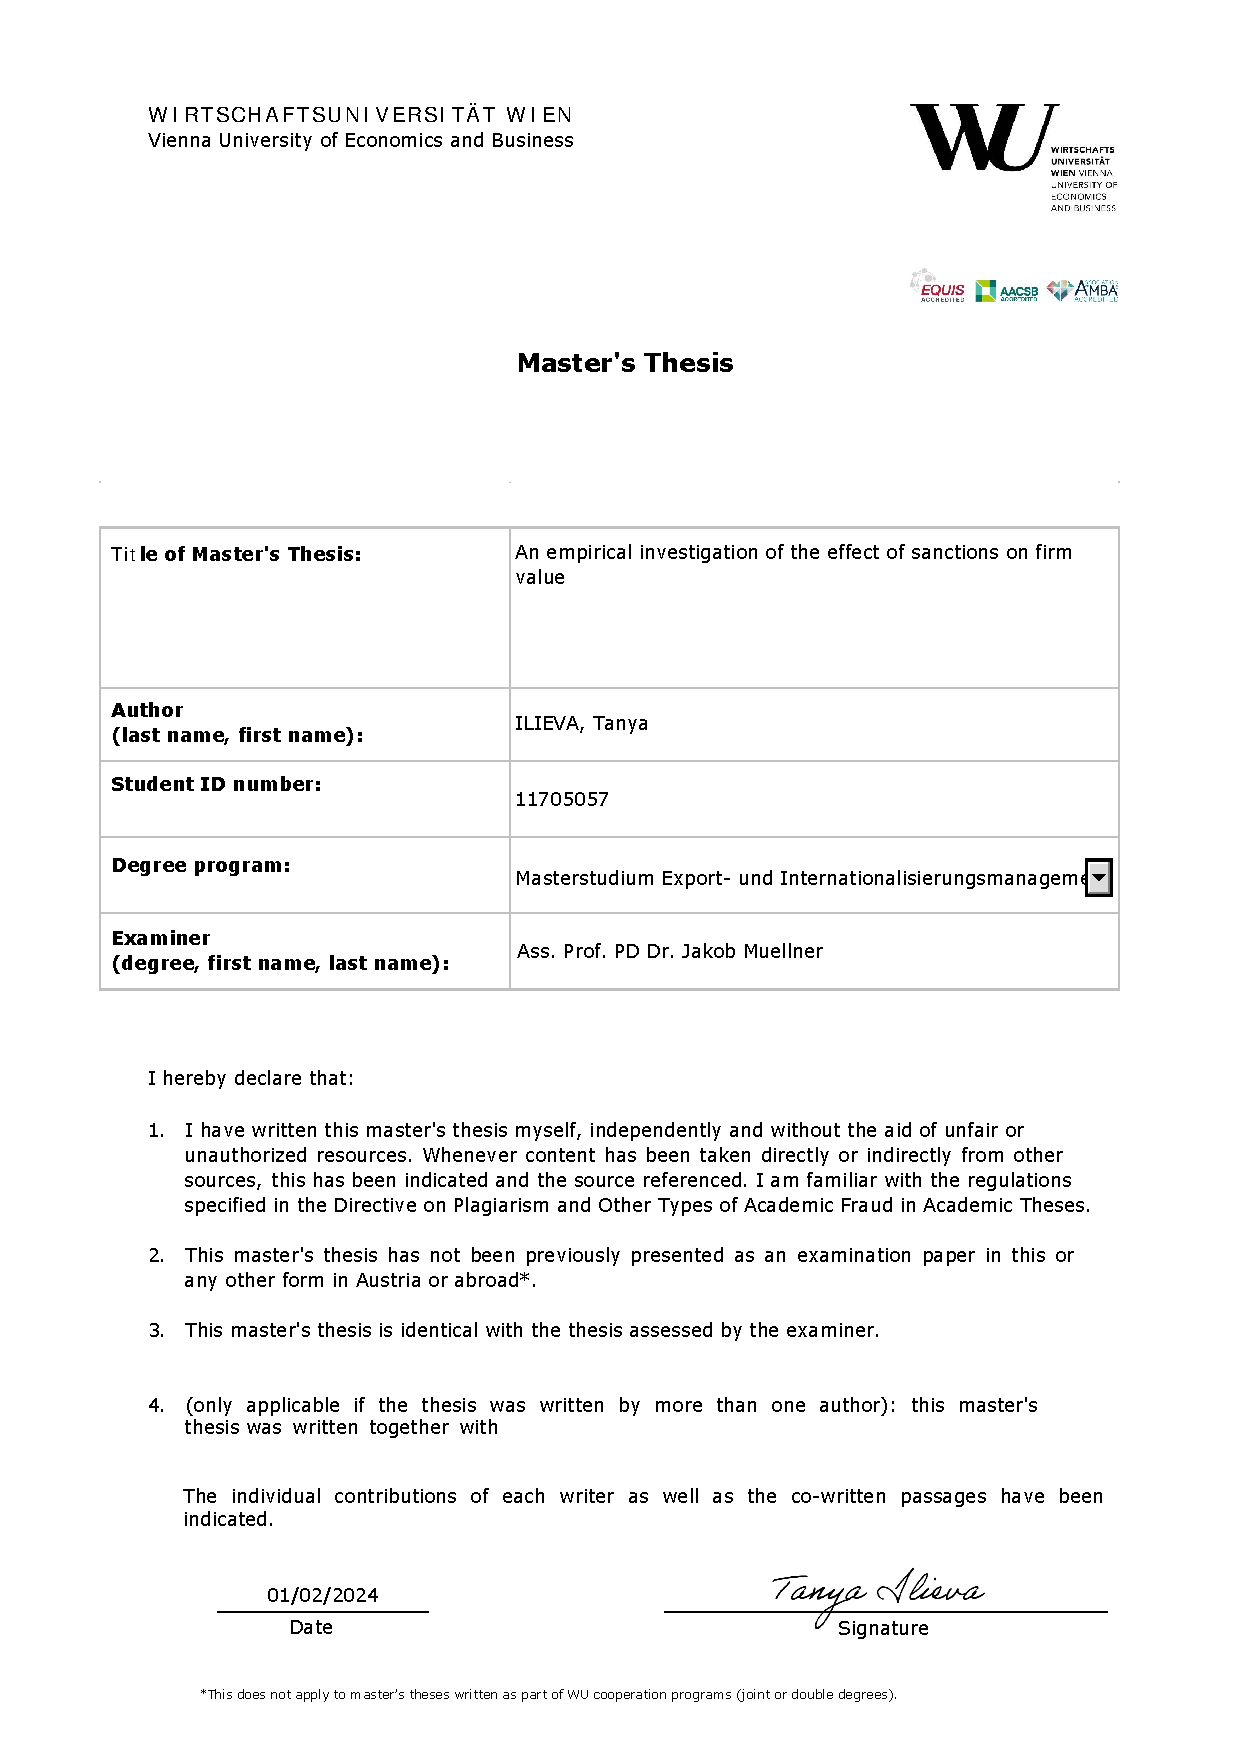
\includepdf[(pages=-]{PDF files/cover.pdf}

\begin{titlepage}
   % \begin{center}
        \Large
        \center
        \textbf{An empirical investigation of the effect \newline of sanctions on public companies}
            \small
            \vspace{0.5cm}
            \newline \textit{Master Thesis}
    \vspace{0.5cm}
    \fontsize{12}{11}\selectfont 
    
    \begin{longtable}{p{0.38\linewidth} p{0.65\linewidth}}
            \\   
            \textbf{Author (last name,\newline first name):} & ILIEVA, Tanya Kirilova\\ 
            \\
            \textbf{Student number:} & 11705057 \\
            \\
            \textbf{Topic:} & An empirical investigation of the effect of sanctions on firm value\\
            \\
            \textbf{Supervisor:} & PhD Anna Andronovich\\
            \\
            %\textbf{Co-Supervisor:} & Ass. Prof. PD Dr. Jakob Muellner\\
            %\\
            \textbf{Examiner:} & Ass. Prof. PD Dr. Jakob Muellner\\
            \\
            \textbf{Department:} & Department of Global Business and Trade\\
            \\
            \textbf{Institute:} & Institute for International Business\\
            \\
            \textbf{University:} & Vienna University of Economics and Business \\
           \\
           \textbf{Date of submission:} & \today \\
           \\
          % \textbf{Note:} & This project proposal aims to summarize important findings about Mercier and the market it operates in. The information is supporsed to be used as a basis for development of a detailed analysis during a block course in winter semester 2023. \\
    \end{longtable}
           
       \vspace{3cm}
       \centering
      
\includegraphics[width=0.1\textwidth]{0. Logos/wu_wien.png} 
       %\begin{figure}
        %   \centering
         %  
\includegraphics[width=0.2\textwidth]{0. Logos/wu_wien.png}
           %\caption{Caption}
           %\label{fig:enter-label}
       %\end{figure}
       % 
      
 \small
        Vienna University of Economics and Business\\
        Vienna, Austria\\
        2024          
%    \end{center}
\end{titlepage}



%%%%%%%%%%%%%%%%%%%%%%%%%%%%%%%%%%%%%%%%%%%%%%%%%%%%
%%%%%%%%%%%%%%%%%%%% lists %%%%%%%%%%%%%%%%%%%%%%%%%
%%%%%%%%%%%%%%%%%%%%%%%%%%%%%%%%%%%%%%%%%%%%%%%%%%%%
\begin{spacing}{1}
\tableofcontents
\end{spacing}

\newpage
\listoftables
\newpage
\listoffigures
\newpage
\fancyhead[RE,LO]{LIST OF ACRONYMS}
\addcontentsline{toc}{section}{List of Acronyms}
\section*{List of Acronyms}
\printglossary[type=\acronymtype, style=twocolumnleft, title={ }]

%\begin{acronym}[CPU]
    \acro{BHAR}{buy-hold abnormal returns}
    \acro{CAR}{cumulative abnormal returns}
    \acro{DID}{Difference-in-difference}
    \acro{EU}{European Union}
    \acro{EBIT}{Earnings before interest and tax}
\end{acronym}
% Give the longest label here so that the list is nicely aligned


%\vspace{-1em}
%\begin{spacing}{0.5}
%    \printglossary[type=\acronymtype, title={}] 
%\end{spacing}

%%%%%%%%%%%%%%%%%%%%%%%%%%%%%%%%%%%%%%%%%%%%%%%%%%%%
%%%%%%%%%%%%%%%%%%%% declaration %%%%%%%%%%%%%%%%%%%
%%%%%%%%%%%%%%%%%%%%%%%%%%%%%%%%%%%%%%%%%%%%%%%%%%%%
%\newpage
%\addcontentsline{toc}{section}{Declaration}
%\fancyhead[RO,LE]{DECLARATION}
%\section*{Declaration}

%The authors hereby declare that:
%\newline

%\indent 1. This case study was written together from Tsveta Hristova und Tanya Kirilova Ilieva. %The individual contributions of each writer as well as the co-written passages have been indicated.
%\newline \indent 2. The authors have written this case study by themselves, independently and without the aid of unfair or unauthorized resources. Whenever content has been taken directly or indirectly from other sources, this has been indicated and the source referenced. The authors are familiar with the regulations specified in the Directive on Plagiarism and Other Types of Academic Fraud in Academic Theses.
%\newline \indent 3. This case study has not been previously presented as part of the competition Case Challenge 2023 at Bank Austria in this or any other form in Austria or abroad.
%\newline \indent 4. This case study is identical with the topic assessed by the Digital Channels teams and communicated in the online video from Nadine Kronlechner and Lukas Mician.

%\fontsize{12}{11}\selectfont 
%    \begin{longtable}{p{0.30\linewidth} p{0.70\linewidth}}
%    \\
%    \\
%    \\
%    \\
%    \\
%    \\
%    \\

%\textbf{Date:} 02.05.2023 & \textbf{Signatures:} \\ 
%&  ~~~~~~~~~~~~~~~~~ Hristova. T.   \\ 
%\\
%&  ~~~~~~~~~~~~~~~~~ Ilieva, T.K.\\ 
%    \end{longtable}

% The data are supporting actors in the story you tell. The lead actors are the questions and the larger issues you are addressing. The story grows from the data, but the data are not the story. (Writing Science, J. Schimel)

%%%%%%%%%%%%%%%%%%%%%%%%%%%%%%%%%%%%%%%%%%%%%%%%%%%%
%%%%%%%%%%%%%%%%% abstract %%%%%%%%%%%%%%%%%%%%%%%%%
%%%%%%%%%%%%%%%%%%%%%%%%%%%%%%%%%%%%%%%%%%%%%%%%%%%%

\newpage
\addcontentsline{toc}{section}{Abstract}
\fancyhead{}
\fancyhead[RE]{ABSTRACT}
\section*{Abstract}
This master thesis examines the impact of restrictive measures (a.k.a. sanctions) on international trade and business from the perspective of European companies. It focuses on the most significant events of announced sanctions by the EU against Russia in 2021, which are used as a signal for potential escalation. The literature review indicates that ...... . This thesis employs an event study by \cite{brown_using_1985} and a regression analysis by \cite{fama_size_1995} to examine the short-term effects of EU sanction announcements on stock prices across a sample of 4.082 Euronext-listed companies. The results show that restrictive measures did have predominantly negative effect of stock prices, especially in ...... sectors. This master thesis contributes to the research in international business and sanctions by providing insights into the consequences of EU sanctions at a detailed industry level.    


Relevance and research gap
\newline
%OLD: Goal: compare the effect of the first EU sanctions package and the effect of the last (16.) EU sanctions  package on the performance of EU based companies 
        %explain in lieu of compare% 
        % definitions:
        %   - first sanction package: wave of sanctions announced between 22.Feb 2022 and 25.Feb 2022
        %   - last sanctions package: wave of sanctions announced between 24.Feb 2025 and 27.Feb 2025
        %   - EU based: companies from the STOXX 600 Index which countries are part of EU;
        %   - EU based: companies from MSCI European Large Cap
        %   - EU companies: EU large-cap companies
        
        % I can do Diff in Diff if my base group is the whole STOXX 600 (large caps) or MSCI European Union Index (large cap) -> NO, we are not conducting a DID analysis
        % If you want an index strictly reflecting EU large-cap companies, MSCI or a customized STOXX Europe index filtered for EU countries is better.
        
%---------------
!!! This list must be deleted before submission !!!
\gls{ai}
\gls{bhar}
\gls{car}
\gls{caar}
\gls{did}
\gls{EU}
\gls{ebit}
%---------------


%Methodology: comparison of linear regression models with different dependent variables for firm valuation (BHR and EBITDA)
%\newline
%Summary of findings
%\newline 
%implications and contributions

\textbf{Keywords:} restrictive measures, sanctions, Russia, conflict, crisis, international business  


%%%%%%%%%%%%%%%%%%%%%%%%%%%%%%%%%%%%%%%%%%%%%%%%%%%%
%%%%%%%%%%%%%%%%%%%% INTRODUCTION %%%%%%%%%%%%%%%%%%
%%%%%%%%%%%%%%%%%%%%%%%%%%%%%%%%%%%%%%%%%%%%%%%%%%%%

\newpage
\fancyhead{}
\fancyhead[R]{\leftmark} 
\section{Introduction}
\label{chap:intro}
\pagenumbering{arabic}
\setcounter{page}{1}


\subsection{Relevance of the topic}
\label{subchap:intro_relevance}\\
With the rise of armed conflicts around the world, the observed trend of de-globalization (e.g. cite A. Mohr) and the consequences of it connected to building blocs of political, economical allies and imposing tariffs and sanctions are becoming an undeniable part of the reality we are living in. A current example of the de-globalization trend is the ongoing tension between the Russian Federation (shortly called Russia in this master thesis) and Ukraine. After the end of the Cold War between the West and the East blocks, although slightly hidden from the masses, the tension has decreased, but never really disappeared. The idea of imposing rules and power over other nations has always been part of the history and it is here to stay. 

Although over the past decades, efforts were made to brings societies together by promoting the process of globalization, hidden figures have been playing in the background, sustaining tension and creating conflict in many geographical areas. And economic scholars do not just observe the environment, but also put effort in building models to analyse it and explain them. In uncertain times, an events like armed conflicts or trade wars might often get visibility. They attract scholar's attention due to the fact that many variables are included and dependencies need explanation. For instance, \cite{gu_how_2021} explains the reaction of the Chinese stock market to external uncertainty in the face of the Sino-US disputes. Another example is coming from \cite{li_china-us_2020} who works on investigating the China-US trade dispute and ist effect on the corporate earning management strategy. Recently, scholars turned to investigating the arised conflict between Russia and Ukraine \citep{assaf_price_2023}. The literature on investigation conflicts and disputes in the world is a common practice and scholars often times focus on exploring the monetisation effect on companies earnings, company activities or company returns. 

As part of the literature on political risks, a subsection dedicated to sanctions, is of special interest to the author of this master thesis. Sanctions are .....   

For the last 10 years, multiple events have been a part of the conflict between Russia and Ukraine. Starting in 2015, relations between the two sides have become increasingly strained. The tension was reflected in acts that led to an armed conflict between the two sides involved. As a response to the decisions made by political figures in the mentioned countries, other major players often tend to impose sanctions in hope of affecting the tense situation. In the case with Russia-Ukraine conflict, the United States of America and the European Union jointly initiated a series of sanctions against the Russian Federation, commencing in February 2022.  These affected actors may either reap benefits or incur detriments from imposed sanctions.  These measures, conceived as strategic responses to the nation's aggressive military maneuvers vis-à-vis Ukraine, aim to erode Russia's standing on the global stage \cite{council_of_the_european_union_eu_2024}. As of the composition of this thesis, the freezing of over EUR 21 billion in Russian assets within the EU, along with the imposition of sanctions amounting to more than EUR 40 billion on exports to Russia and exceeding EUR 90 billion on Russian imports to the EU, attests to the magnitude and economic ramifications of these punitive actions. An overview of the sanctions from Feb 2022 until Feb 2024 are included in \ref{overview_sanctions}.  


\subsubsection{Practical Relevance}
\label{subchap:intro_relevance_practical}
%  \item stats about the santions imposed to other countries in the last three years

% \item we live in a world full of sanctions, so we need to know what we are doing
Finally, sanctions are being imposed on other countries as well. Based on the \cite{} there are sanctions imposed, for instance, on Iran or North Korea. This comes to show that sanctions are relevant for international business and exploring the effects of sanctions on listed companies that operate in a global environment can bring new knowledge and deepen understanding of global processes and dependencies. 

%  \item stats about the santions imposed to Russia in the last three years
 In a short time period of twelve months the European Commission agreed on imposing ten packages of massive and unprecedented sanctions against the Russian Federation with the aim of weakening the country position on the global scene "in response to the military aggression against Ukraine" \cite{council_of_the_european_union_eu_2024}. At the point of writing this theses, over EUR 21 billion Russian assets had been frozen in the EU, more than 40 billions of exports to Russia and over 90 billion Russian imports to EU sanctioned so far. Even though the sanctions have impact on all parties involved, the European Union considers a new set of sanctions against China and India in 2024 \cite{noauthor_eu_nodate}. 
 
%\item relevant for international companies
Moreover, companies exposed to sanctions need to bear the economic and reputational losses. In the year 2020, ...... of the international trade of the EU was conducted with Russia, whereas four years later, the numbers look differently, namely .... . More than 8.000 European companies were affected by the desicions of imposing sanctions on one of the largest economies in the world. These companies need to consider a series of potential strategies such as staying, exiting, or adapting, in the uncertain business environment that they have to operate in. 



% \item book connection: Sanctions have been a part of the world for decades and this is why they have such an important role in the world order today. They are mainly part of the policy instruments used by governments who want to rule the world. These are not only important for decision making and block-building, but also for creating allies and non-allies among nations worldwide. Thus, in the newest events sanctions have played a crutial role in the new conflicts that arose in the last three years around the globe. And they will continue to play an important role in the world for upcoming conflicts especially in the Asian countries. But how to manage sanctions? What is their role for large enterprises and international companies that need to play on the dangerous field between governments, policy, economy and personal interest in the face of higher financial return?
%\end{itemize}

%EPU/PPIP/BERI index
Explain that the economic policy uncertainty index (EPU index) shows that there is an increased risk in Russia compared to other countries. "The EPU index is a commonly used indicator to measure uncertainty. Baker et al. (2016) compile the economic policy uncertainty index by using newspaper report frequency. They search the articles of the top ten news media in the United States by keyword retrieval, and then calculate the number of keyword articles to the total number of newspapers and periodicals published, and finally obtain the economic policy uncertainty index." (Gu et al., 2021, p. 3) \citep{gu_how_2021}
%https://www.policyuncertainty.com/all_country_data.html
\begin{figure}
    \centering
    \includegraphics[width=0.5\linewidth]{Images/EPU Russia.png}
    \caption{Economic Uncertainty Index (EPU) for Russia}
    \label{fig:epu_russia}
\end{figure}

\ref{fig:epu_russia} shows that the initial large increase in the economic uncertainty index for Russia occurs in 2020. However, literature puts less emphasis on this moment and the events connected to Russia during that period.

As of 2026, people live in a global world that is highly dependable on resources, policies and economic developments. Thus, empirically exploring the nature of sanctions and their effect on firm value in the past has a pivotal role in the fields of politics, economics and international business. The topic of sanctions has practical, empirical and theoretical relevance at the time of this research. In the next subsections each of these three directions of relevance will be explained in more details.   \ac{bhar}  \cite{abbassi_what_2022}

\subsubsection{Empirical Relevance - empirical papers}
\label{subchap:intro_relevance_empirical}
The database of the World Bank shows that there have been more than 1000 sanctioned comapanies and individuals over the last 24 years. International companies and national companies looking to expand are facing more and more restraints and sanctions from institutions worldwide. 

As of 2025, most academic research in the field of international business and sanctions focused on analysing the effect of the Russia-Ukraine conflict on various stakeholders, especially around February 2022. Most authors accept that the beginning of the military conflict between the two countries begins on February 24, 2022 \citep{ } . They identify it based on articles of world-leading financial newspapers and renowned magazines. The author of this master thesis conducted independent research using the database Factiva to confirm the information. However, some authors use a different date as a robustness check for their empirical results. There is a lack of research in the time before Feb2022. It is believed that events before the actual military event start, can be used as an indicator for the following events. In this master thesis, we will focus on sanction imposition against the Russian federation prior to the conflict outbreak in Feb2022. We want to find out the most significant events prior to the war start that might have effected companies returns and evaluate the reaction of the market to these events. f

So far, researchers have explored the effect of the war by using the event method. Some have focused on the imposed sanctions from different countries. However, most studies are country-level oriented \citep{assaf_price_2023, boubaker_heterogeneous_2022, tee_financial_2023, sonnenfeld_it_2022, kamal_impact_2023, kumari_are_2023} , where the variables in the regression are macro-level data such as GDP, Export, Import and other macroeconomic identifiers. The first  study that focused on exploring firm-specific variables Federle et al. (2022) provide first firm-level evidence. They find that particularly firms that are geographically closer to Ukraine experience more severe share price losses. ; 
was conducted by \cite{abbassi_what_2022}. After that, \cite{sami_exploring_nodate} conducted a firm-level analysis for MENA countries. \cite{kumari_are_2023}'s study is the one focusing on European markets. They measure the market by using MSCI index and compare its performance to individual stocks of 25 EU countries. 

While most published studies focus on the event dates in February 2022, this master thesis aims to explore the effect of imposed sanctions by the European Union on companies' performance listed on Euronext Stock Exchange.   


"While most prior studies focus on the short-term price reaction of national stock market indices around the outbreak of the armed conflict between Russia and Ukraine, observing large declines (e.g., Boungou and Yati ́e, 2022; Yousaf et al., 2022), Federle et al. (2022) provide first firm-level evidence. They find that particularly firms that are geographically closer to Ukraine experience more severe share price losses. We aim to examine whether this initial market reaction may help to explain a firm’s decision regarding its Russian operations." \citep[p.~3]{kiesel_should_2023}


Among the recent major political risk events, Smales (2017) documents a significantly positive relationship between political risk (the Brexit referendum) and financial market uncertainty. He et al. (2017) examine the economic cost of non-violent diplomatic disputes between mainland China and Taiwan and show that political tension is related to a significantdecline in stock market returns. \citep{kamal_impact_2023}

Prior studies show that political events and the associated uncertainty have a considerable impact on stock returns and volatility (He et al., 2017 ; Smales, 2017; Bash and Alsaifi, 2019; Hillier and Loncan, 2019; Buigut and Kapar, 2020; Kapar and Buigut, 2020; Ahmed et al., 2022; Boubaker et al., 2022). Some studies document that negative stock market reactions to political uncertainty persist in the post-eventperiod (He et al., 2017). \citep[p. ~4]{kamal_impact_2023}

\citep{kiesel_should_2023} expose the effect of a stay or leave decision in Russia to companies returns. "We observe positive stock returns to leave decisions (+0.67 \% during the three days surrounding the announcement), but do not find any significant reaction for stay decisions." 


\begin{itemize}
  \item relevance 1: G7 analysis 
  \item relevance 2: new dataset 78.000 data points-> manually constructed
  \item relevance 3: new way to measure Russian exposure -> in contrast to \citet{balyuk_divesting_2023} who uses numerical firm-leveled data such as "revenues, sales, assets, and similar data, which we then scaled using respective per-war metrics for the entire firm", we offer to measure the Russian exposure on the basis of intensity of discussions to leave/stay/adapt the market 
  \item show how the term sanctions has been used in papers over time 
\end{itemize}



\subsubsection{Theoretical Relevance - philosophical papers}
\label{subchap:intro_relevance_theoretical}

\begin{itemize}
 \item the negative stock market impact is not solely driven by the threat of violence but also by economic penalties targeting selected businesses \citep{he_hurting_2017}
  \item relevance 1: institutional theory perspective \cite{peng_toward_2023}
  Having outlined the institution-based view’s three major criticisms, next we showcase four promising research directions: (1) deglobalisation and sanctions. Such institutional transitions naturally trigger changes in firm behaviour, which will have signifcant performance implications (Yiu et al., 2018).  Instead of being some interesting events only affecting emerging economies, institutional transitions are likely to become the “new normal” throughout the world (Ahlstrom et al., 2020; Li et al., 2022). Therefore, as a dynamic theory built around the interaction between institutions and organisations (Peng, 2002), the institution-based view will become more important.the advancement of the institution-based view in the scholarly world and its development in the wider world in the last two decades, during which the only constant seems to be institutional change
  As a result, much of the research on institutions focuses on innovation (Khoury & Peng, 2011; Zhou et al., 2017), market entry (Boddewyn & Peng, 2021; Deng et al., 2020; Lu et al., 2018; Meyer et al., 2009; Yiu & Makino, 2002), and growth of the frm (Peng & Heath, 1996; Peng et al., 2018a). In contrast, there is little research on sanctions, withdrawals, and shrinking of the frm, to name a few. Defned as “the process of weakening economic interdependence among countries” (Witt, 2019: 1054), deglobalisation seems to be a new wave that has hit the world (Peng et al., 2021; Petricevic & Teece, 2019). Evidence of deglobalisation is everywhere: border closures, COVID-induced lockdowns, immigration controls, investment screenings, military conficts, nationalism, sanctions, supply chain localization, and trade wars. How managers and frms respond strategically to such changing rules of the game has presented a series of new research opportunities (Ahlstrom et  al., 2020; Contractor, 2022; Globerman & Shapiro, 2009; Peng & Kathuria, 2021; Peng et al., 2021; Rodrik, 2018; Young et al., 2022). This can become a new research frontier in the institution-based view (Li et al., 2022). Among numerous topics on deglobalisation, an institution-based view can inform research on sanctions. The recent scale, scope, and frequency with which sanctions are imposed is unprecedented. Sanctions can be defned as politically motivated, nonmilitary coercive measures against foreign countries, organizations, and/or individuals (Bapat & Kwon, 2015; Meyer et al., 2022; Mirkina, 2018). Sanctions are key tools of foreign policy, and the West has long imposed sanctions on smaller countries such as Cuba, Iran, Myanmar, and North Korea (Meyer & Thein, 2014). Now larger countries such as China and Russia are frequently targeted, and these countries have launched countersanctions against the West. Yet, “our theoretical understanding of sanctions is woefully underdeveloped” (Felbermayr et al., 2021: 2). Consider Western multinational enterprises (MNEs) operating in Russia since its February 2022 invasion of Ukraine. For foreign frms operating in Russia whose home-country governments are imposing sanctions on Russia, the strategic choices include: (1) permanent withdrawal, (2) temporary closure, and (3) business as usual. In contrast to the tremendous amount of work in the institutions literature on legitimisation, the process of delegitimisation has rarely been studied (Oliver, 1992). Essentially, if MNEs choose options 1 and 2, they lose legitimacy in the eyes of host-country stakeholders in Russia. But if they choose option 3, they lose legitimacy in the eyes of stakeholders in the home country and third countries (Stevens et al., 2016). Given the thorny nature of each option, the strategic choices are not preordained, thus necessitating more in-depth research. A new generation of research on the institution-based view can leverage the imprinting of the new era (Barry & Kleinberg, 2015; Li et  al., 2022; Luo, 2022; Meyer & Li, 2022; Witt, 2019; Witte et al., 2020). Fascinating but underexplored questions in a new institution-based view of deglobalisation and sanctions include: How predictable are government actions (Witt, 2019)? How maneuverable is corporate diplomacy (as opposed to country diplomacy) (Li et al., 2022)? How can MNE subsidiaries engage with local stakeholders to minimize the impact of sanctions (Meyer \& Li, 2022)? Given the global nature of deglobalisation and sanctions, this new area of research can address Criticism 1 by demonstrating that the institution-based view is a globally relevant paradigm.
  \item relevance 2: operational flexibility and real options theory 
\end{itemize}

\subsection{Research questions}
\label{subchap:intro_question}

\begin{description}
   \item[Research Question 1:]  What theories effectively explain the effects of internationalisation as a possible resilience determinant?
\end{description}

\begin{description}
   \item[Research Question 2:]  What are the current state and main insights of the research on Sanctions against the Russian Federation and their impact on companies and companies resilience to black swan events?
\end{description}

\begin{description}
   \item[Research Question 3:]  How did the announcement of the European Union's second package of sanctions against Russia affect the market value of European publicly listed firms, and to what extent did the magnitude of the market reaction vary with firms' exposure to Russia? 
\end{description}

%\begin{description}
%   \item[Research Question:]  What is the effect of sanctions on firm value?
%\end{description}
%it contributes to : evaluation of financial sanctions \cite{ghasseminejad_impact_2021}




  \subsection{Methodology}
\label{subchap:intro_methodology}
The scientific design begins with a review of relevant literature and appropriate theories. This step aims to answer the first two research questions. On the one side, it ensures a deep dive into the academic knowledge available in the field of sanctions against the Russian Federation. On the other side, it summarises the theoretical basis used in the field of complexity science, catastrophes, and black swan events in international business. Due to current inconsistencies of theory on internationalisation as a company resilience determinant and the gap in the academic literature on sanctions in international business, the emphasis of the research lies on a comprehensive selection of the used sources. This approach aims to deliver a well-structured qualitative overview of the latest state of research on the topic. Furthermore, it promises reliable insights into the main focus points of theoretical and empirical findings. Hence, the primary focus lies on published academic sources, credible electronic databases, reliable statistics sources and recognised high-quality journals for gathering sufficient information to complete the literature screening. 

For to identify relevant academic literature a bibliometric database approach was chosen, as proposed by \cite{hiebl_sample_2023}. The selected database was \textit{Scopus}. As of September 2023, \textit{Scopus} is being described as "the largest abstract and citation database of peer-reviewed literature: scientific journals, books and conference proceedings" (cited on their \href{https://service.elsevier.com/app/answers/detail/a_id/15100/supporthub/scopus/}{own website}). Delivering a thorough overview of the world's research output in multiple fields such as social sciences, medicine, technology, and arts and humanities, \textit{Scopus} features smart tools to track, analyse and visualise research. Due to its large scope of journals and highly-developed functions, \textit{Scopus} is the most sophisticated and most appropriate database at the time this master thesis was written. The main objective of reviewing academic articles 1) to summarise relevant theories that focus on company resilience in term of internationalisation and 2) to illustrate the current state of research and thus provide solid basis on the subject if the sanction impact on companies. Main criteria for the choice of articles was developed on basis of the approach proposed by \cite{tuselmann_revisiting_2016}. The research was further enhanced by the use of novice tools that make accurate recommendations based on a network approach. Moreover, the institute's journal ranking served as a supplementary source of information. At last, popular economic journals such as Harvard Business Review, The Economist, and Handelsblatt, as well as the latest reports from the European Commission and the World Bank, are monitored for the latest updates on the situation. Leveraging this dual-tiered approach ensured a rigorous selection of literature for the study.  

%Initially, a qualitative study grounded in a comprehensive literature review was conducted. This methodological approach facilitated the identification and collection of pertinent articles and publications germane to the study. To ensure a meticulous search, databases were thoroughly selected from the WU Catalogue based on their relevance. 

%The research encompassed the following steps. First, to streamline the search process, relevant keywords were employed, including  \textit{sanction*}, \textit{firm OR corporate valu*}, \textit{firm OR corporate performance}. An extension of these important keywords was conducted by requesting machine learning generating programs to suggests example keywords for a literature search \footnote{See Appendix.}. More than twenty terms were proposed. However, these suggestions were not used in the next steps. 

%Second, the first relevant keywords that were identified, were used to conduct an advanced search in ProQuest database. Moreover, judicious use of connectors such as OR, AND within the database was employed in order to optimize search efficiency. Preference was given to publications with relevnce to the topic of the master thesis, WU-star ranking, and \cite{tuselmann_revisiting_2016}'s ranking whenever feasible. The WU Vienna's list of starred journals comprises highly reputable and dependable sources readily accessible to students, whereas \cite{tuselmann_revisiting_2016} developed a highly-reliable ranking of the journals with the use of an empirical approach.  

%database-driven approach \citep{hiebl_sample_2023} for sampling literature reviews AND
%enriched by the use of Inciteful.xyz \citep{library_using_nodate}
%\begin{itemize}
%    \item bibliometric database Scopus 
%    \item selection criteria
%    \begin{itemize}
%        \item impact factor or JCR-indexed journals with an IF above a given threshold, e.g. 1.0 plus following
%        \item restriction to 40 papers 
%        \item keywords can be found in the title, abstract, list of keywords, and full text of the article 
%        \item time scope 2013-2023 -> matches the dataset -> "important to cover at least a bare minimum of a 10 year period for a systematic literature review" \cite{paul_art_2020}
%        \item 
%    \end{itemize}
%\end{itemize}
%Moreover, the institute's journal ranking served as a supplementary source of information. Leveraging this dual-tiered approach ensured a rigorous selection of literature for the study. Additionally, the author scrutinized references within relevant articles and other notable works, harnessing them as valuable resources for further exploration and augmentation of the academic discourse.



With regard to the quantitative part of the master thesis, the focus was on gathering secondary data from various databases. 

LSED databases for earnings calls, ORBIS database for company-level data, \href{https://sanctions.ddns.net/}{Sanctions Dashboard from the International Business Institute at WU Vienna}, Wharton Database for independent variables were preferred. In order to measure the immediate effect of the sanctions on the companies' stock prices and to answer the third research question, a new sample of 1.800 companies with a measured Russian exposure and the event study methodology was used. The preferred data on the individual companies for the implementation of the event study methodology are daily/monthly/quarterly adjusted closing prices/buy-hold returns, which are obtained from Bloomberg/Refinitiv/Wharton database. This statistical method supports the analysis and measurement of significant stock prices' reactions, so called cumulative abnormal returns (CAR), to the announcement of a black swan event, in this case, events' announcements related to sanctions against the Russian Federation. The event study methodology is deemed to be practical and useful for the estimation of the effect an unanticipated event can have on the firms' prices in international markets. \cite{brown_using_1985} define the event study methodology as a statistical approach that focuses on "the impact of particular types of firm-specific events on the prices of the affected firms' securities". Additionally, numerous scholars such as \cite{abbassi_what_2022}, \cite{assaf_price_2023}, \cite{ghasseminejad_impact_2021} and \cite{kiesel_should_2023} the event study methodology in their research connected to the role of sanctions against the Russian Federation in various event windows. Overall, event studies are often times preferred by scholars to measure and graphically illustrate the effects of an unanticipated event on the value of companies and investors.


\subsection{Thesis Structure}
\label{subchap:intro_thesisstructure}
The initial section of this thesis serves the purpose of furnishing an introductory framework for the chosen subject matter. This segment not only delineates the research questions and hypotheses but also provides a concise overview of the employed methodology.

The second section is dedicated to a comprehensive review of pertinent literature. Commencing with a succinct introduction to the field of behavioural economics, the subsection culminates with an elucidation of key findings from the literature, striving to establish cogent connections between various articles.

The third section meticulously details the chosen methodology. It commences with an exposition on the acquired data, followed by a comprehensive description of the study's sample. The subsequent elucidation pertains to the presentation of variables, encompassing dependent, independent, and control variables. Concluding this section is the explication of the empirical model, followed by a meticulous breakdown of the results derived from the conducted analysis.

The fourth section of this master thesis encapsulates a summary of the study's findings, offering a critical discussion thereof. Additionally, this segment acknowledges extant limitations inherent in the empirical study and proffers avenues for prospective research. Lastly, the conclusion delves into potential implications for both theory and practical application.






%%%%%%%%%%%%%%%%%%%%%%%%%%%%%%%%%%%%%%%%%%%%%%%%%%%%%%%%%%%%%%%%%%%%%%%%%%%%%%%%%%%%%%%%%%%%%%%%%%%
%%%%%%%%%%%%%%%%%%%%%%%%%%%%%%%%%%%%%%%%%%%%%%%%%%%%%%%%%%%%%%%%%%%%%%%%%%%%%%%%%%%%%%%%%%%%%%%%%%%
%%%%%%%%%%%%%%%%%%%%%%%%%%%%%%%%%%%%%%%%% MAIN PART OF THE THESIS %%%%%%%%%%%%%%%%%%%%%%%%%%%%%%%%%
%%%%%%%%%%%%%%%%%%%%%%%%%%%%%%%%%%%%%%%%%%%%%%%%%%%%%%%%%%%%%%%%%%%%%%%%%%%%%%%%%%%%%%%%%%%%%%%%%%%
%%%%%%%%%%%%%%%%%%%%%%%%%%%%%%%%%%%%%%%%%%%%%%%%%%%%%%%%%%%%%%%%%%%%%%%%%%%%%%%%%%%%%%%%%%%%%%%%%%%
\section{Theory Review}
\subsection{Efficient Market Hypothesis} - because we assume that the price reflects the market; The market should react quickly to the information, and the price adjustment should occur around the event.
\subsection{Markowitz portfolio diversification theory} - because we are building a portfolio of the equivalent of the STOXX600 (benchmark)  
\subsection{Political Risk Theory}
\subsection{Behavioural Finance Theory} - Use this to explain possible deviations from the EMH and potentially unexpected/persistent market reactions.

\subsection{Hypothesis development}

\section{Literature review}
Following \citep{hiebl_sample_2023}

“After the exclusion process, we proceeded to an additional verification step by conducting an ancestry search (Aguinis et al., 2011), reviewing the reference lists of the current selection of articles.” (Nielsen et al., 2023, p. 2) \citep{nielsen_disasters_2023}

following \citep{paul_art_2020} we create a visual representation as part of a bibliometrical review in the field of international business

\subsection{Hypotheses formulation}

\cite{aria_bibliometrix_nodate}

Proposition 1: Managers and companies rationally pursue their interests and make strategic choices within the formal and informal constraints in a given institutional
framework.
Proposition 2:  While formal and informal institutions combine to govern firm behaviour, in situations where formal constraints are unclear or fail, informal constraints will play a larger role in reducing uncertainty, providing guidance, and conferring legitimacy and rewards to managers and firms.

\begin{figure}[ht]
  \centering
  \includesvg[width=1\textwidth]{Images/Literature.drawio}
  \caption{Event Timeline with 140 *** days of estimation period and 21 *** days of event window including anticipation and adjustment windows}
  \label{es_graph}
  \DeclareGraphicsExtensions{.svg}
\end{figure}

\cite[p.~19]{kiesel_should_2023} use Sanctionscanner to identify relevant events. In this master thesis, the source of information for sanctions is chosen to be the EU Sanctionsmap \footnote{https://www.sanctionsmap.eu/#/main}.  
\citep[p.~3]{kumari_are_2023} follow the PIIE to identify sanctions https://www.piie.com/blogs/realtime-economics/2022/russias-war-ukraine-sanctions-timeline

The event had a significant negative impact on the average returns of all firms.

\begin{description}

\item[\emph{Hypothesis 1:}]
The announcement of EU sanctions against Russia resulted in statistically significant negative cumulative abnormal returns for STOXX Europe 600 constituent firms.

\item[\emph{Hypothesis 2:}]
Firms with greater economic exposure to Russia experienced more negative cumulative abnormal returns following the announcement of EU sanctions against Russia.

\item[\emph{Hypothesis 3:}]
The magnitude of cumulative abnormal returns following the announcement of EU sanctions against Russia differs significantly across industries, with firms in more sanctions-sensitive industries experiencing stronger negative abnormal returns.

\end{description}

\section{Methodology}

Economists often focus on measuring and explaining impact of various changes in the environment on different variables. One of the moThe event study methodology has been more significantly used in recent time and argued to be among the best methods to examine the impacts of extreme events (Bekiros et al., 2017; Boubaker et al., 2015; Hassan et al., 2022a,b; Pandey and Kumari, 2021a,b; Rai and Pandey, 2021; Zoungrana et al., 2021). 


The main references with regards to the methodology used for event studies was layed out by MacKinlay, 1997 and Brown and Warner, 1980 and 1985. Years later, scholars have been doing literature reviews on event studies with the aim of summarising best practices and structuring useful knowledge. One of the recognised summaries of the event study methodological practices comes from  Kothari and Warner, 2004. They are not only giving the technical overview of performing an event study, but also focus on answering the question "how to best specify and test interesting economic hypotheses using event studies", p.6. 


%-> MacKinlay (1997) and Campbell, Lo, and MacKinlay (1997) document the origins and breadth of event studies.
-> The relation of event studies to tests of market efficiency receives considerable attention in Fama (1991)
-> Smith (1986) presents reviews of event studies of financing decisions
-> Jensen and Ruback (1983), Jensen and Warner (1988) and Jarrell, Brickley and Netter (1988) survey corporate control events

->the basic statistical format of event studies has not changed over time. It is still based on the table layout in the classic stock split event study of Fama, Fisher, Jensen, and Roll (1969). The key focus is still on measuring the sample securities’ mean and cumulative mean abnormal return around the time of an event.
-> daily/inraday returns preferred over monthy returns
-> more sophisticated methods when it comes to long-horizon event studies - also coming in paralel with th edevelopments in the asset pricing literature, particularly the Fama-French-3 factor model

-> we can have more confidence and put more weight on the results of short-horizon tests than longhorizon tests, p.9 Kothari and Warner
-> Short-horizon tests represent the “cleanest evidence we have on efficiency” (Fama, 1991, p.1602)
-> sample size and firm characteristics are extremely important for the plausibility and the power of the event study p.15-19
-> 

All event studies, regardless of horizon length, must deal with several basic issues. These include risk adjustment and expected/abnormal return modeling (Section 4.2), the aggregation of security-specific abnormal returns (Section 4.3), and the calibration of the statistical significance of abnormal returns (Section 4.4).

Brown and Warner (1985) conclude that simple risk-adjustment approaches to conducting shortwindow event studies are quite effective in detecting abnormal performance.

The question of which model of expected returns is appropriate remains an unresolved, contentio us issue. , p.25

Regardless of whether the \textbf{size}, \textbf{book-to-market}, and \textbf{momentum factors proxy for risk }or indicate \textbf{inefficiency}, it is essential to use them when measur ing abnormal performance, p.25-26

Abnormal performance measurement: 
-> characteristic-based matching approach (BHAR approach) , p.26 Kothari - Mitchell and Stafford (2000, p. 296) describe BHAR returns as "the average multiyear return from a strategy of investing in all firms that complete an event and selling at the end of a prespecified holding period versus a comparable strategy using otherwise similar nonevent firms.” ; 
For BHAR, researchers have developed:
(1) bootstrap (Lyon te al, 1999) - 1. calculate skewness-adjusted t-statistic, 2. cpnstruct a bootstrapped distribution of the adjusted t-statistic and 
(2) pseudoportfolio-based statistical tests that might account for the cross-correlations and lead to accurate inferenes
-> Jensens's alpha approach (calendar-time portfolio approach), p.26


When it comes to long-horizon event studies in the recent years, researchers have put effort into solving this problem, e.g.: 
As of per Goldsmith-Pinkham and Lyu, 2025 causal inference can be stimated as part of an event syudy in three ways:
"(1) classic abnormal return estimators, based on specified factors, 
 (2) difference-in-mean estimators, which construct control groups through decisions of the econometrician, and 
 (3) synthetic estimators (Abadie \& Gardeazabal, 2003; Abadie et al., 2010), which use historical prices from control assets to construct either a replicating portfolio (synthetic control) or to construct a set of factors using PCA (Xu, 2017)."

"The key insight is that rather than imposing a specific factor structure ex ante (applicable for CARs), the synthetic methods construct a portfolio of control securities that best match the pre-event return path of treated securities. If such a replicating portfolio exists, it should provide valid counterfactual returns in the post-event period without requiring correct specification of the underlying factor model." - Goldsmith-Pinkham and Lyu, 2025



Pros:
-> 

Cons: 
-> "buy-and-hold abnormal return estimates are particularly challenging to estimate because they require the matching portfolio to not just match on expected returns, but also on volatility. If the control group’s returns have different variance, then the differing volatility drag will lead to very different results"; "doing buy-and-hold abnormal returns with an index can be seriously flawed. "  - Goldsmith-Pinkham and Lyu, 2025




The data for the regression analysis is taken from three different databases. First, a street view earnings calls data was retrieved from the Refinitiv database. Second, performance indicators measured as long-term event abnormal returns were obtained via the Wharton Database. Third, firm-level covariates were collected via the ORBIS Database. Finally, data points from the three datasets were merged and cleaned. 

\textbf{Refinitiv:} More than 70.000 observations about earnings calls from publicly listed companies were downloaded from Refinitiv. The data was cleaned by a professional analyst. Based on the text analysis it was possible to evaluate companies that have been discussing Russia-Ukraine situation over a period of 10 years, from 2013 to 2023. This data indicates the intensity of discussions with regards to each country and intensity of discussions of three types of strategy decisions of executives.

%Based on the text analysis each data point was evaluated in three aspects, namely sanctions exposure degree, sanctions exposure type and sanctions response.

\textbf{Wharton Database/Yahoo Finance/Orbis?:} BHAR, stock prices, indices 


\textbf{Orbis:} The list included 76.988 observations and 26 variables. After the data was analysed in R, was made clear that the dataset contains information about 14.698 companies in a time period from 2013 to 2023. Unfortunately, not all companies were present in each year. In order to develop a trustworthy dataset with relevant and equally-distributed information, companies which were not present in all years during the given time span, were subtracted. Thus, after filtering for appropriate observations, the final list of companies in the dataset equalled 2.374 companies. As stated by \cite{sonnenfeld_it_2022}, ORBIS contains data on legal entities in Russia, similar to the data from EGRUL  

\textbf{European commission}: data on sanctions
\subsection{Sampling procedures}
Which particular firms were targeted and which were eventually included in the study?
% OLD
%The original sample of the companies for the quantitative study was deducted by using a dataset from \href{https://www.lseg.com/en/data-analytics/financial-data/company-data/events/earnings-transcripts-briefs/transcripts-database}{LSED Transcripts \& Briefs Database}. LSED Transcripts are deemed to be a verbatim representation of institutional and corporate events. These are considered true transcripts, representing exactly what is heard during the event. The provided summaries are unbiased and condensed versions of a transcript such as M\&A Calls, Sales Calls, Earnings Calls, Analyst Meetings and Corporate Presentations. Summaries provide a snapshot through a financial table and identify key figures and themes discussed in a given transcript. The database provides company coverage for 10,000 companies including all major global indices such as the S\&P 500 and Russell 100, the first data originating from 2001. The original sample included all companies which published earnings calls information between 2013 and 2023. As some companies became part of or were removed from the LSED dataset during the chosen time frame, the sample was considered as not fully reliable. That is why by using coding in R, only companies that provided full information of earnings calls between 2013 and 2023 were deemed acceptable matches for the sample that we use in this qualitative study. Thus, the sample was restricted to 2.374 companies whose earnings calls were included in the LSED dataset between 2013 and 2023 and have available data on their earnings calls. However, not all companies were exposed to the Russian sanctions directly. That is why the criteria for exposure was decided to be "positive Russian or Ukrainian count" in the dataset, meaning that the companies were actively discussing a situation connected to one of these countries. As a result, the final dataset consists of ..... companies. 

%The sample was compared to samples of previous studies that is the KSE Institute database \citep{kiesel_should_2023}. This dataset is based on Yale's School of Management List of companies \citep{sonnenfeld_it_2022}. Due to that fact, there is about 99\% overlap of the information between the KSE dataset and the other datasets, with the main difference being that the KSE dataset is more developed. This dataset applied a thorough methodology from \cite{mylovanov_how_2023} that was developed in more than a year with the help of various experts. The methodology is very detailed and reliable. \cite{kiesel_should_2023} develops a new dataset that relies on the information from the KSE dataset, but focuses only on companies that have already gone through an IPO and are being traded on an international stock exchange. He identifies 1.281 relevant firms. That is why the author of the Master thesis decided to compare the LSED dataset with the \cite{kiesel_should_2023}'s dataset for potential overlaps. This comparison is going to ensure a level of compatibility and will create a basis for discussion on data similarities. 

The dataset consists of 4082 companies. Within these companies, 2830 were found in Orbis and had a recognizable BvD Ids.   

From the comparison, it is evident that .....

As a result, the final sample is set to include ..... number of companies. 


 \subsection{Study design}
“Event study methodology is an empirical method often used by scholars in the financial field. It is used to study the impact of a specific event on the stock price or yield of a company, and to test the response of financial market to new information disclosure. According to the duration of events, event study methodology is usually divided into daily event study and long-horizon event study (\citep{brown_using_1985}; Fama, 1991). In the field of corporate finance, the daily event study provides a good indicator to measure the impact of an event on shareholders’ wealth, that is, Cumulative Abnormal Returns (CARs). The daily event study mainly focuses on the announcement effect within a few days around the event announcement day, which provides relevant evidence for investors to understand the company’s dividend allotment, merger and acquisition decisions (e.g., Edmans, 2011; Deng et al., 2013). In additionto corporate events, some scholars use the event study methodology to study the impact of non-corporate events on crude oil or stock prices.” 
Liu et al. (2020a, 2020b, 2020c) examine the impact of COVID-19 on China’s and global stock index returns, and observes the reactions of different industries in China using the data of stock returns at firm level, and find that the stock markets in China and the Asia region have suffered the most severe impact. Demirer and Kutan (2010) study the impact of OPEC and SPR announcements on crude oil prices from 1983 to 2008, and find that only OPEC’s announcements of production reduction can cause significant statistical asymmetric impact, while SPR announcements are more short-term effect. We use similar approaches to comprehensively analyze the information effect in Sino-US disputes. ([Gu et al., 2021, p. 4] \citep{gu_how_2021}

The standard market model event study "...is commonly used in the related literature on military conflicts and the impact of stock returns on firm decisions (see e.g., Wiles, Morgan, and Rego, 2012; Giammarino et al., 2004; Boubaker et al., 2022; Guidolin and La Ferrara, 2007). \citep[p.~8]{kiesel_should_2023} %In further robustness tests, we calculated abnormal returns using a multifactor model, a market-adjusted model and a generalized autoregressive conditional heteroskedasticity (GARCH) market model that includes autoregression and moving average (ARMA) terms. The robustness checks indicate that our results are not likely to be influenced by our methodology for measuring abnormal returns.\citep[p.~8]{kiesel_should_2023} 
 
\cite{he_covid19s_2020} and \cite{bhattacharjee_cross-border_2025} choose to organise the study designs with a 140-day estimation window. The large number of days is evaluated to be the most suitable time window for two reasons. First, the choice of a 140-day estimation window yields a higher possibility of reducing bias in the historical data and forecasts based on it compared to shorter estimation periods. Second, the large estimation window is considered to avoid the lack of reliability in the results. That is why, for this work, an estimation window of 140 days will be applied in the study design.

There is a gap of *** time to avoid the bias of the estimation window on the specified event window. The event window is divided into two parts - Anticipation Window or the pre-event duration and the Adjustment Window or post-event duration (shown in \ref{es_graph}).

for estimating the expected returns with a 225-days estimation window [−230,−6]10 and a 36-days event window [−5,+30].11 \citep[p.~3]{kumari_are_2023} 

%Comment on SVG importing: sensitive to small and large letters!
\begin{figure}[ht]
  \centering
  \includesvg[width=0.8\textwidth]{Images/eventstudy}
  \caption{Event Timeline with 140 *** days of estimation period and 21 *** days of event window including anticipation and adjustment windows}
  \label{es_graph}
  \DeclareGraphicsExtensions{.svg}
\end{figure}


\begin{figure}[ht]
  \centering
  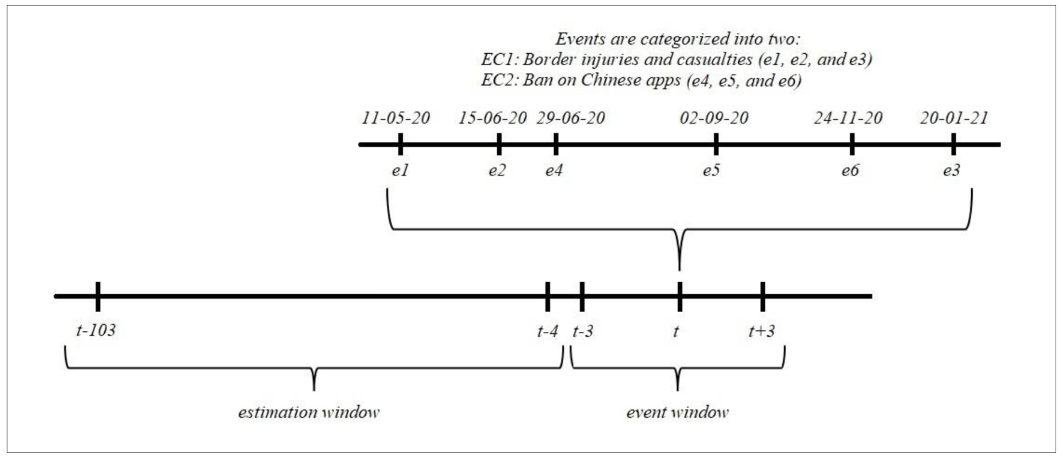
\includegraphics[width=0.8\textwidth]{Images/hassan_2022.png}
  \caption{Event Timeline Hassan et al (2022)}
  \label{es_graph}
\end{figure}

\begin{figure}[ht]
  \centering
  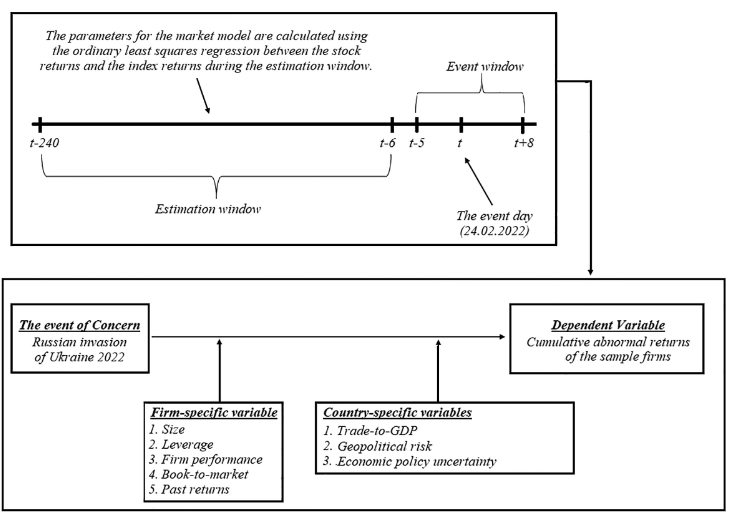
\includegraphics[width=0.8\textwidth]{Images/abbassi_2022.png}
  \caption{Event Timeline \cite{abbassi_what_2022}}
  \label{es_graph}
\end{figure}

\begin{figure}[ht]
  \centering
  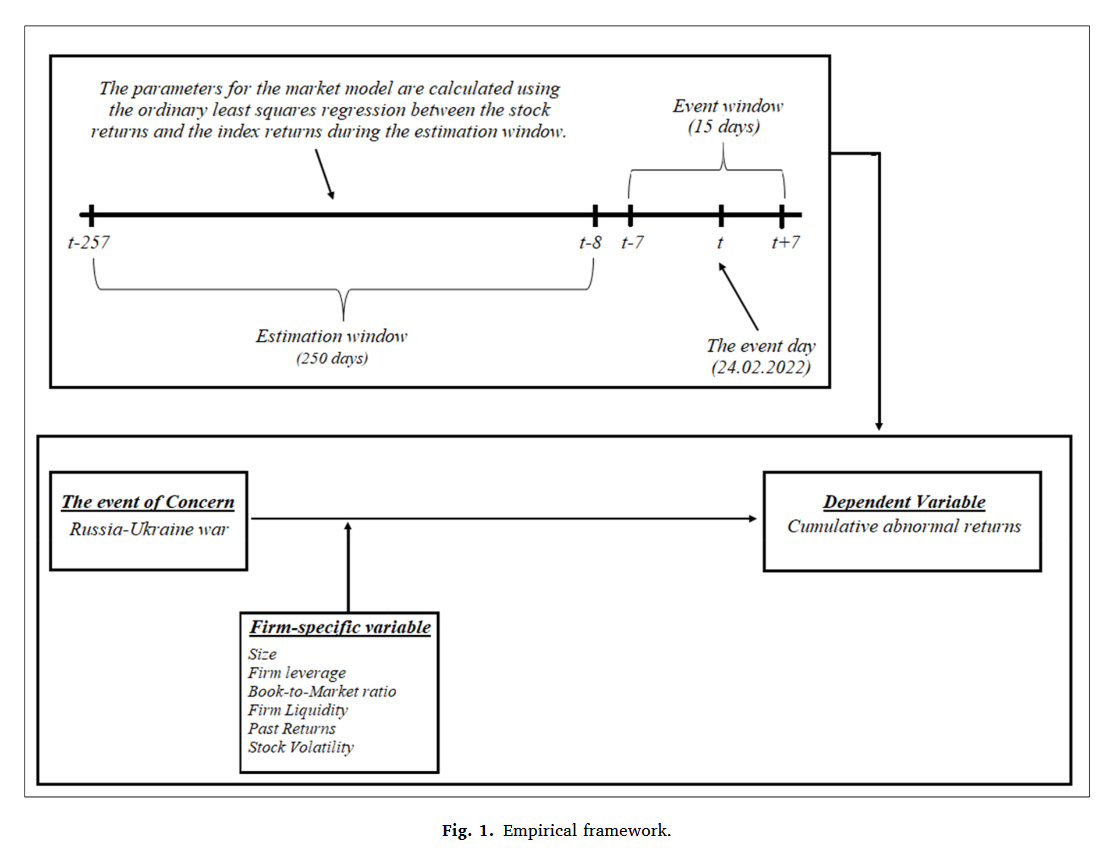
\includegraphics[width=0.8\textwidth]{Images/pandey_2023.png}
  \caption{Event Timeline \cite{pandey_border_2023}}
  \label{es_graph}
\end{figure}


Similar to \cite[p.5]{abbassi_what_2022} and \cite{pandey_border_2023}, we build the empirical framework showing the dependencies between dependent, independent and control variables \textbf{(check the slides from Zapkau for a deep dive and ideas to expand this paragraph!)}  

Chaturvedula et al. (2015), Pandey and Kumar (2022b), and Boubaker et al. (2022) evidence that past returns are capable of predicting cumulative abnormal returns. Hence, we use past returns (PAST) as a control variable. \citep[p.~3]{kumari_are_2023}

We are planning to measure the effect on the European market as of three dates that are identified as important:


\begin{table}[h!]
\centering
\begin{tabular}{@{}llc@{}}
\toprule
\textbf{Date} & \textbf{Event Description} & \textbf{Use as Event Date?} \\
\midrule
April 9, 2021   & First reported Russian military movement       & Yes \\
Nov 22, 2021    & Confirmation of renewed military movement      & Yes \\
Dec 17, 2021    & Issuance of security proposal to NATO          & Yes \\
Feb 24, 2022    & Start of Russian military operation            & \textcolor{red}{No} \\
\bottomrule
\end{tabular}
\caption{Event Dates and Their Relevance}
\label{tab:event_dates}
\end{table}

\begin{table}[h!]
\centering
\begin{tabular}{@{}llcl@{}}
\toprule
\textbf{Window} & \textbf{Dates} & \textbf{Days}& \textbf{Notes} \\
\midrule
Estimation      & 1 Jul 2021 – 17 Dec 2021       & 120  & Normal returns estimation; avoids prior events \\
Gap             & 18 Dec 2021 – 11 Feb 2022      & 35   & Avoids contamination from anticipatory market reactions\\
Event           & 14 Feb 2022 – 18 Mar 2022      & 25   & capturing market reaction to the event\\
\bottomrule
\end{tabular}
\caption{Summary Table for CAR Measurement (21 Feb 2022)}
\label{tab:event_dates}
\end{table}

Which data were collected and when?
The data focuses on large corporations listed on the European Stock Exchange, known as Euronext. Established in 2000 through the consolidation of the Amsterdam, Brussels, and Paris stock exchanges, Euronext has since expanded its operations to include markets in Portugal, Ireland, Italy, and Norway. It represents the largest stock exchange in Europe by market capitalisation, with a total value of approximately \$7.2 trillion, positioning it among the top five global exchanges. The competitive landscape of Euronext includes major regional exchanges such as the London Stock Exchange Group and Deutsche Börse, as well as international entities such as the New York Stock Exchange and NASDAQ. Its role in improving market integration, investor access, and financial innovation underscores its significance in the broader context of global financial markets. 
The data was gathered in August 2025 and focuses on publicly traded companies in Europe that are listed on Euronext. The daily returns were extracted with a Python code from Yahoo Finance for a time frame that ensures at least 140 days estimation window .  

\textbf{Was a control group used?}
In this study, a control group is not included primarily because the Russia-Ukraine conflict represents a large systemic shock affecting global markets broadly. Consistent with the methodology of many event studies analyzing major crises—such as the global financial crisis or pandemics—this research relies on established benchmark models, like the market model and Fama-French factors, to estimate normal and abnormal returns. These models effectively capture expected returns based on market-wide and factor-based risks, allowing for the isolation of abnormal performance without the need for a separate control group. This approach is well-supported in the literature when the event under study has pervasive market effects that limit the identification of truly unaffected firms.


\textbf{Were the data collected at different levels of analysis?}
This study utilizes data collected across multiple levels of analysis to capture the complexity of the Russia-Ukraine conflict’s impact on Euronext-listed companies. The primary data are at the \textbf{firm level}, including daily stock prices, returns, and financial characteristics necessary for calculating cumulative abnormal returns. To better understand firms’ direct exposure to the conflict, information on the \textbf{number and location of subsidiaries} was gathered, providing a subsidiary-level dimension of geographic exposure. Additionally, \textbf{sector classifications} were incorporated to control for industry-specific effects and to explore variation across economic sectors. Finally, \textbf{market-level data} such as overall market returns and risk factors from the \textcolor{red}{Fama-French model} (https://mba.tuck.dartmouth.edu/pages/faculty/ken.french/data_library.html) were used as benchmarks in the estimation of normal returns. By integrating data from firm, subsidiary, sector, and market levels, this study offers a comprehensive and nuanced analysis of abnormal stock returns in response to geopolitical events.

Was the design more suitable for theory development or theory testing?
theory testing: portfolio theory, financial flexibility theory, real-options theory,
complexity theory: seems nice and mathematically based


Was the design experimental or quasi-experimental?
The research design is quasi-experimental in nature, as it analyzes the impact of an exogenous geopolitical event (the Russia-Ukraine conflict) on stock returns of Euronext-listed firms without any random assignment. The event serves as a natural experiment, and abnormal returns are estimated using the Fama-French 3-factor model.

This study analyzes the impact of the Russia-Ukraine conflict on publicly listed companies using data from the Euronext exchange, which includes firms across several European markets. Stock-level daily return data were collected for all Euronext-listed companies during both the estimation window and the event window. The Fama-French 3-factor model was applied to estimate expected returns, using European factor data (Market-RF, SMB, and HML) and the corresponding risk-free rate. Given the short-term nature of the event study and the regional context, the 3-factor model was preferred over the 5-factor version to avoid overfitting and to ensure robustness, as the additional factors (profitability and investment) are less reliable in non-U.S. settings and less relevant for short-window abnormal return analysis. Euronext was chosen for its cross-country coverage and market relevance within the European economic space.

The abnormal return ARi,t on a distinct day within the event window represents the difference between the actual stock return Ri,t on that day and the normal return expected given the capital asset pricing model (CAPM) relation in the absence of the sanctions announcement. (from Jakob)

Was the design inductive, deductive or abductive?
%deductive research tests a theory by building hypotheses and planning a research strategy 

The study adopts a deductive research design, beginning with established financial theories regarding market efficiency and asset pricing (e.g., the Fama-French model) and applying these to test empirically whether abnormal returns around the Russia-Ukraine conflict varied among Euronext-listed firms.


\textbf{1. Estimate Normal Return Model (Estimation Window)}
\begin{equation}
R_{i,t} - R_{f,t} = \alpha_i + \beta_i^{\text{MKT}} (R_{m,t} - R_{f,t}) + \beta_i^{\text{SMB}} \cdot \text{SMB}_t + \beta_i^{\text{HML}} \cdot \text{HML}_t + \varepsilon_{i,t}
\end{equation}

Abnormal returns (AR) and cumulative abnormal returns (CAR) ``are calculated following \cite{brown_using_1985}: 

\begin{equation}
AR_{[t_0-n, t_0+n]} = R_{it} - (\alpha + \beta*R_{mt})
\end{equation}

The abnormal return $AR_t$ is typically calculated as:

\begin{equation}
AR_t = R_t - E[R_t]
\end{equation}

where:
\begin{itemize}
    \item $R_t$ is the actual return at time $t$,
    \item $E[R_t]$ is the expected (normal) return at time $t$.
\end{itemize}

\begin{equation}
{AAR} = \frac{1}{N} \sum_{i=1}^{N} AR_i  
\end{equation}

The Cumulative Abnormal Returns (CAR) over a time window from $t_0-n$ to $t_0+n$ are calculated as:

\begin{equation}
CAR_{[t_0-n, t_0+n]} = \sum_{t=t_0-n}^{t_0+n} AR_{it}
\end{equation}

where:
\begin{itemize}
    \item $CAR_{[t_0-n, t_0+n]}$ is the cumulative abnormal return over the event window $[t_0-n, t_0+n]$,
    \item $AR_t$ is the abnormal return at time $t$,
    \item $n$ is the number of days for which the estimation period is being set. It can take the values 2, 5, 10, 20, and 50.  	
\end{itemize}


\begin{equation}
{CAAR} = \frac{1}{N} \sum_{i=1}^{N} CAR_i  
\end{equation}

similarly to \citep[p.~1]{kumari_what_2022}, we use a cross-sectional regression to explore the connections between event-led abnormal returns and the listed firm characteristics. 
\subsection{Data}
panel dataset 
Euronext companies
4079 companies listed
2830 companies Orbis
\textcolor{red}{2759} companies with full data


\subsection{Variables}
\subsubsection{Dependent Variable}

Performance metric - Long-Term Event Abnormal Returns;
Buy-hold return - the market determines the price of the stock  how the market thinks the company will perform; 

longrun event study 180 days , but we have annual data, ideally 360/365 days or annual buy-hold returns; Wharton Database; at the same time do a long run measure EBIT or EBITDA vs. how the company will perform; If the two are slightly different you can reflect how severe this company would be affected 
2020-2022
%2013-2023

\subsubsection{Independent Variable}
\begin{itemize}
  \item total assets
  \item roe
  \item Tobin's Q
  \item nr of employees
  \item ebit margin
  \item industry
  \item nr of all subsidiaries 
  \item nr of subsidiaries in Russia
  
  \item sanctions exposure degree, define types of sanctions EU Commission, identify the most significant ones 
  %\item sanctions response, from the earnings calls dataset
  %\item financial aid for Ukraine
\end{itemize}


\subsubsection{Control Variables}
covariates vs. factors 

what could moderate the negative effect on a company in Russia, e.g. Microsoft is international and it has less OR having a company in turkey could be less
invasion is on 24. Feb 2022 
always from 24. Feb in 180 days periods
for every year we have 2 BHAR and the most important are the first 180 days after the conflict 

\section{Statistical Modelling}
regression analysis was used as a basis for evaluating the hypotheses in the master thesis:
\begin{equation} \label{lin_reg_bias}
	f(x) = {x_0\beta_0 +x_1\beta_1 +x_2\beta_2 + ... +\epsilon} 
	\end{equation}
where \textit{f(x)} is the dependent variable.
conduct a parametric and non-parametric tests! 

\subsection{Robustness check/Sensitivity analysis}
Although the parametric t-value has been shown to yield better results with the market model, the significance of the test results is not affected due to the non-normality of the daily returns (Brown and Warner, 1985; Dyckman et al., 1984). To confirm whether the results may change using a non-parametric test of significance, however, we use the Corrado (1989) test. \citep[p.~12]{kumari_what_2022}



\subsubsection{Parametric tests}
As a robustness check, a parametric t-test was conducted, following the example of \cite{boubaker_heterogeneous_2022} and \cite{ghasseminejad_impact_2021}. 

t-statistics including 3, 5, 7 and 10 days around the event date at aggregate level \citep[p.~6]{gu_how_2021}
t-statistics including 3, 5, 7 and 10 days around the event date at disaggregate level \citep[p.~7]{gu_how_2021}

t-value for testing the statistical significance \citep[p.~3]{hassan_border_2022}

a t-test is applied to the cross-sectional standardized daily abnormal returns (SARs) and standardized cumulative abnormal returns (SCARs) for individual and multiple event days, respectively. \citep[p.~5]{kamal_impact_2023}

“we utilize the standardized cross-sectional test of \citep{boehmer_event-study_1991}(henceforth the BMP test) to test the significanceof the average AR and CAR.“For this purpose, first, we standardize the ARi and CARi using the estimation window standard deviation.” \cite[p. ~5]{kamal_impact_2023}

we use the parametric t-test \citep[p.~8]{kiesel_should_2023}

the parametric test provides stable results irrespective of the data being normal or abnormal (Brown and Warner, 1985; Dyckman et al., 1984) \citep[p.~10]{kumari_are_2023}

statistical significance is assessed using the t-statistic described in Kothari and Warner (2007). \citep[p.~499]{omar_diversifying_2017}

%\subsubsection{Measurement of abnormal returns based on Index?}

%\subsubsection{Difference-in-difference test (DID)}
We do not use a differnce-in-difference test, because it is hard to find a peer group that is not directly or indirectly affected by the observed geopolitical changes.  
%\subsubsection{Placebo test}

\subsubsection{Non-Parametric tests}
As a robustness check, we calculate the \cite{corrado_nonparametric_1989} value (a non-parametric rank test) for the event-wise AARs, as modified by Ataullah et al. (2011): 
\begin{equation}
    C = \sqrt{\frac{3}{N(T^2-1}}*\sum_{i=1}^{n} [2K(AR_{it} - (T-1)] 
\end{equation}

where, C is the \cite{corrado_nonparametric_1989} value, N is the sample size (i.e., the number of global stock market indices), T is the total number of days, including the estimation and event window (146 in our case),K (ARit) is the rankof the abnormal return of the index i in the 146 days. The Corrado values (Table 6) depict similar results as in Table 3. \citep[p.~8]{boubaker_heterogeneous_2022}

We follow Ataullah et al. (2011) to calculate the Corrado (1989) value (C) \citep[p.~3]{hassan_border_2022}

we supplement our parametric tests with the non-parametric Wilcoxon signed-rank test to determine whether the median of the abnormal cross-sectional return is statistically significant \citep[p.~5]{kamal_impact_2023}

we use ..... and the Wilcoxon rank-sum test \citep[p.~8]{kiesel_should_2023}

In further robustness 1tests, we calculated abnormal returns using a multifactor model, a market-adjusted model and a generalized autoregressive conditional heteroskedasticity (GARCH) market model that includes autoregression and moving average (ARMA) terms. The robustness checks indicate that our results are not likely to be influenced by our methodology for measuring abnormal returns.\citep[p.~8]{kiesel_should_2023}

we conduct the Corrado (1989) test as modified by Ataullah et al. (2011), which is a non-parametric test of significance of the abnormal returns \citep[p.~10]{kumari_are_2023}

\subsubsection{Measurement of abnormal returns based on BHAR}
Following \citep{gu_how_2021}, we estimate the average buy-and-hold abnormal returns (BHAR) for robustness check. We employ BHAR methodology and replace CAR:
\begin{equation}
BHAR_{c,-T,T} = 
\left[ \prod_{t=-T}^{T} \bigl(1 + R_{ct}\bigr) -1 \right] -
\left[ \prod_{t=-T}^{T} \bigl(1 + E(R_{ct})\bigr) \right]
\end{equation}
“Where BHARc, T1, T2 is the BHAR for event c over an interval of trading days starting with day T and ending with T; Rct is the actual realized return for event c at time t calculated by Fama-French model; and E(Rct) is theexpected return. We also compute the t-statistic for the average BHAR and CAR over a particular event window.” \citep{gu_how_2021}, p.5

\begin{equation}
\text{BHAR}_{i}[0, +250] = 
\frac{\sum_{t=0}^{250} (1 + R_{it})}{\sum_{t=0}^{250} (1 + M_{Rt})}
\end{equation}
\citep[p.~6]{xu_trade_2021}

\subsubsection{Measurement of abnormal returns with different dates}
“As discussed in Section 2.1, following prior studies (e.g., Ahmed et al., 2022), we use February 22, 2022 as the event date to examine the impact of the Russia–Ukraine crisis on Australian stock returns. One may argue that the start of the war itself is more important than the recognition of the break-away regions. To check the sensitivity of our analysis, in this section, we use the actual invasion date (i.e., February 24, 2022) as our event day. This event day is consistent with earlier studies (e.g., Boubaker et al., 2022). We use the same research methods as used for our main empirical estimation.” \citep[p,~15]{kamal_impact_2023}


with a shorter 135day estimation window \citep[p.~10]{kumari_are_2023}
\section{Limitations}
\label{chap:limitations}

\begin{itemize}
  \item time frame 
  \item size of sample
  \item chosen performance measure - abnormal returns, not CFs, revenue, etc.
  \item dataset includes only public companies
  \item small and medium enterprises are not included in the analysis 
  \item use another method to calculate the effect of sanctions, e.g. look at  \cite{gonzales_martinez_apocalypse_nodate}
  \item although Euronext is considered to be the largest stock exchange in Europe with roughly \$7 trillion market capitalization, companies listed on the LSE, Deutsche Boerse or SIX might enrich the dataset and bring new insights to the research world
\end{itemize}

\section{Further research}
\label{chap:further}
Further research will encourage IB society to better understand the effect of sanctions on firms. The first proposal is to calculate the "response surface of the IB catastrophe model of firm performance as \cite{gonzales_martinez_apocalypse_nodate} explain it for COVID-19 firms in Europe. This will allow the IB society to illustrate " the effects of X traditional determinants of firm performance and black swan shocks related to the grand challenges in global business (Z)" \citep{gonzales_martinez_apocalypse_nodate}. It will allow a fresh glimpse on the situation from a catastrophe theory perspective, a unique view that is often being overlooked.  

Additionally, it would be useful for future research to investigate the extent to which different industries are directly impacted by Russia-Ukraine and neighboring European countries (such as Germany, Poland, Romania, and the Baltic nations) through trade or investment.\citep[p.~16]{kamal_impact_2023

\subsubsection{Review of empirical research}












\section{Conclusion}
The findings have important implications for policymakers, investors, and researchers.






















%%%%%%%%%%%%%%%%%%%%%%%%%%%%%%%%%%%%%%%%%%%%%%%%%%%%
%%%%%%%%%%%%%%%%% Bibliography %%%%%%%%%%%%%%%%%%%%%
%%%%%%%%%%%%%%%%%%%%%%%%%%%%%%%%%%%%%%%%%%%%%%%%%%%%
\newpage
\bibliographystyle{agsm}
\bibliography{references_zotero}

\newpage
\appendixpage
\addappheadtotoc
\begin{appendix}

\section{SCOPUS Search String as of 20.02.2024}
\begin{lstlisting}[title = {SCOPUS String}, label={scopus_string}, language=R, caption=SCOPUS String]
TITLE-ABS-KEY ( ( sanction* OR "politic* connect*" ) AND ( "cumulative abnormal return" OR "network theor*" ) ) AND PUBYEAR > 2012 AND PUBYEAR < 2025 AND ( LIMIT-TO ( EXACTKEYWORD , "Political Connections" ) OR LIMIT-TO ( EXACTKEYWORD , "Event Study" ) OR LIMIT-TO ( EXACTKEYWORD , "Network Theory" ) OR LIMIT-TO ( EXACTKEYWORD , "Cumulative Abnormal Returns" ) OR LIMIT-TO ( EXACTKEYWORD , "Network Analysis" ) OR LIMIT-TO ( EXACTKEYWORD , "Social Networks" ) OR LIMIT-TO ( EXACTKEYWORD , "Event Studies" ) OR LIMIT-TO ( EXACTKEYWORD , "Abnormal Returns" ) OR LIMIT-TO ( EXACTKEYWORD , "State-controlled Firms" ) OR LIMIT-TO ( EXACTKEYWORD , "Social Network Theory" ) OR LIMIT-TO ( EXACTKEYWORD , "Social Network" ) OR LIMIT-TO ( EXACTKEYWORD , "Sanctions" ) OR LIMIT-TO ( EXACTKEYWORD , "Political Ties" ) OR LIMIT-TO ( EXACTKEYWORD , "Actor Network Theory" ) OR LIMIT-TO ( EXACTKEYWORD , "Invasion Of Ukraine" ) OR LIMIT-TO ( EXACTKEYWORD , "Political Connection" ) OR LIMIT-TO ( EXACTKEYWORD , "War" ) OR LIMIT-TO ( EXACTKEYWORD , "Russian Federation" ) OR LIMIT-TO ( EXACTKEYWORD , "China" ) ) ->37 papers
\end{lstlisting}


\begin{landscape}
\newpage
\section{Literature review}
\begin{spacing}{0.8}
\fontsize{6}{10}\selectfont
\begin{longtable}[c]
{
p{0.06\linewidth} %Author 
p{0.15\linewidth} %Title
%p{0.02\linewidth} %Year
p{0.15\linewidth} %Source Title
%p{0.04\linewidth} %Class
p{0.10\linewidth} %Conflict
p{0.11\linewidth} %Time window
p{0.15\linewidth} %Method
p{0.15\linewidth} %Data
}
\caption{Literature overview}
\label{literature_overview}
\\
\hline
  \textbf{Author} & 
  \textbf{Title} & 
  %\textbf{Year} & 
  \textbf{Source title} & 
  %\textbf{Class}\footnote{Based on the classification of \cite{paul_art_2020}: TM - theory-based; MB - method-based; DB - domain-based; MAB - meta analytically-based} & 
  \textbf{Conflict} & 
  \textbf{Time Window} & 
  \textbf{Method} & 
  \textbf{Data} \\ 
\hline
  \endfirsthead
  \cite{abbassi_what_2022} %Author 
  & What makes firms vulnerable to the Russia–Ukraine crisis? %Title
  %& \citeyear{abbassi_what_2022} 
  & The Journal of Risk Finance 
  %& Class? 
  & Russia-Ukraine, 2022 
  & 02.03.2021 - 08.03.2022
  %examining the impact of the war on the firms of stock market indices of the G7 countries 
  & event study; cross-sectional analysis of \gls{car} &
  \textbf{531 firms} from G7 countries; Refinitiv; \textbf{country-} and \textbf{firm-specific} variables \\
  % We are the first to report firm-level evidence of the Russia–Ukraine war effects (2) Firms in France and the United States are unaffected (3) Stock prices are fragile to geopolitical risks and considerable dependence on trade (4) Higher book-to-market exposes the firms to the risk of exogenous shocks (5) Smaller firms outperform large firms in the G7 stock markets
  %\hline
  %\cite{ahmed_is_2023} 
  %& Is geopolitical risk interconnected? Evidence from Russian-Ukraine crisis 
  %& \citeyear{ahmed_is_2023} 
  %& The Journal of Economic Asymmetries 
  %& ? 
  %& Russia-Ukraine, 2022 & 
%  examines the interconnectedness in the global equity markets during the Russia-Ukraine crisis; has removing Russia from the global equity markets brought any changes to the network & 
  %sample of 27 global equity markets, which included 17 developed, nine developing, and an actor nation (i.e., Russia). 
  %& network theory \\
  % & Despite the fact that removing Russia from the system does not significantly alter network properties, there is a great deal of variation in network properties before and during the war, indicating that the conflict has indirectly caused structural changes in the equity markets. First, the Russia-Ukraine war brings compactness to the global equity market highlighting the characteristics of a denser network during a geopolitical chaos. Second, Russia bringing inactiveness in the equity market network indicating that the presence of a war-hit nation reducesthe activity in the market. Third, a war-hit nation tends to get isolated in the global equity market networkduring geopolitical turmoil. Fourth, the constructed NENI index will enable regulatorsto gauge the position of their stock market performance during a geopolitical crisis.
  \hline
  \cite{assaf_price_2023} 
  & The price of war: Effect of the Russia-Ukraine war on the global financial market 
  %& \citeyear{assaf_price_2023} 
  & The Journal of Economic Asymmetries 
  %& ? 
  & Russia-Ukraine, 2022 
  & dd.05.2021 - dd.03.2022
  & event study; global stock market; the cross-sectional variation in \gls{car} 
  & 65 countries indices; \textbf{country-specific} variables \\ 
  % We find that stock indices show the negative AARs and CAARs after the announcement of the invasion. However, the magnitude of negative return varies for different regions. The developed countries experienced more negative price reactions than emerging countries. In addition, EMEA (Europe, Middle East, and Africa) is the most affected area on a geographical division basis, whereas the American division does not show significant price reactions. Further, countries with higher GDP experi enced less sell-off in their indices. We also find that the trade-to-GDP ratio negatively impacts the abnormal returns in the post-event window, indicating that countries with more percentage of the trade in their GDP have been affected to a greater extent.
  \hline
  \cite{balyuk_divesting_2023} 
  & Divesting under Pressure: U.S. firms’ exit in response to Russia’s war against Ukraine 
  %& \citeyear{balyuk_divesting_2023} 
  & Journal of Comparative Economics 
  %& ? 
  & Russia-Ukraine, 2022 
  & 01.01.2022 - 21.04.2022
  & event study; regression analysis
  & 630 US companies with Russian presence (manual); firm- and industry-specific \\ 
  % When U.S. firms announce exits from Russia in the aftermath of the invasion, there are no adverse announcement effects on their returns. Instead, exit announcements are preceded by a negative trend in abnormal returns that ends immediately on the day of the announcement.
  \hline
  \cite{boubaker_heterogeneous_2022} 
  & Heterogeneous impacts of wars on global equity markets: Evidence from the invasion of Ukraine
  & Finance Research Letters 
  & Russia-Ukraine, 2022 
  & 07.10.2021 - 07.03.2022
  & event study; regression analysis
  & 47 country indices; country-specific \\ 
  \hline
  \cite{ghasseminejad_impact_2021} 
  & The impact of financial sanctions: The case of Iran 
  & Journal of Policy Modeling 
  & U.S.-Iran, until 2013 
  & 2011-2016 
  & event study with \gls{bhar}; 
  & 350 companies on the \gls{tse}; firm-specific variables \\
  \hline
  \citeauthor{gu_how_2021} 
  & How do investors in Chinese stock market react to external uncertainty? An event study to the Sino-US disputes 
  & Pacific-Basin Finance Journal 
  & Sino-US, 2019 
  & dd.10.2017 - dd.08.2020
  & event study
  & index returns on the Chinese stock market (SSEC, SZCS and CSI300) \\
  \hline
  \cite{hassan_border_2022} 
  & Border disputes and heterogeneous sectoral returns: An event study approach & Finance Research Letters
  & Sino-Indian disputes, 2020 
  & 03.12.2019 - 25.01.2021
  & event study; cross-section of the cumulative abnormal returns
  & 8988 observations of daily returns of the 14 NIFTY sectoral indices from the \gls{nse} over six events \\ 
  \hline
  \cite{kamal_impact_2023} 
  & The impact of the Russia-Ukraine crisis on the stock market: Evidence from Australia 
  & Pacific-Basin Finance Journal 
  & Russia-Ukraine, 2022 
  & 14.01.2025 - 29.03.2025 
  & event study by Fama et al. (1969); February 22, 2022 as the event date
  & 295 constituent stocks of the ASX300 index and their \gls{gics} \\
  %\textbf{robustness}: alternative event day; & 
  %behavioural theory (investor's reaction); economic theory (inverse relationship between political risk and stock returns) \\ 
  % Findings: We find significantly negative abnormal returns on the event date (i.e., the first trading day after Russia recognized the two Ukrainian states as autonomous regions) in the Australian stock market. However, this negative stock market reaction mostly disappeared in the post-event period. We also find that small and medium-sized firms were adversely affected during the pre-event and event periods. Interestingly, the magnitude and the direction of the abnormal returns vary across industries. We also find that high-growth, illiquid and export-oriented firms are more exposed to the Russia–Ukraine crisis.
  % Future Research: We suggest that future studies could utilize industry-specific import and export data to provide a more detailed examination of cross-industry effects. Additionally, it would be useful for future research to investigate the extent to which different industries are directly impacted by Russia-Ukraine and neighboring European countries (such as Germany, Poland, Romania, and the Baltic nations) through trade or investment.
  \hline
  \cite{kiesel_should_2023} 
  & Should I stay or should I go? Stock market reactions to companies' decisions in the wake of the Russia-Ukraine conflict 
  & Journal of International Financial Markets, Institutions and Money 
  & Russia-Ukraine, 2022 
  & 01.01.2022 - 30.04.2022
  & event study 
  & 1281 firms from KSE Institute and Refinitiv database traded on an international stock exchange \\ 
  % We observe positive stock returns to leave decisions (+0.67 % during the three days surrounding the announcement), but do not find any significant reaction for stay decisions. We provide evidence that leave decisions are announced earlier if the initial share price reaction to the outbreak of the armed conflict was more pronounced, indicating that investors may appreciate a clear commitment to exit the Russian market. The results do not indicate that firm decisions (leave or stay) are based on previous stock returns, but we find that firms with larger negative returns at the beginning of the conflict obtain more positive returns around the firms' decision announcements. Finally, we show that firms that change their initial decision are more likely to opt to leave the Russian market than to stay.
  \hline
  \cite{kumari_are_2023}  %VERY GOOD ONE
  & Are the European Union stock markets vulnerable to the Russia–Ukraine war? 
  & Journal of Behavioural and Experimental Finance 
  & Russia-Ukraine, 2022 
  & 17.03.2021 - 11.04.2022
  & event study by \cite{brown_using_1985} with the market model; 36 days event window; 225 days estimation window; event day 24.02.2022
  & MSCI EUROPE as benchmark + 25 EU countries; country-level analysis  \\
  %\textbf{robustness} check: shorter 135day estimation window and the non-parametric test of "Corrado (1989) as modified by Ataullah et al. (2011)" 
  
  % Findings: We find adverse event day impact on the stock market indices. Further, Poland, Denmark, and Portugal exhibit positive cumulative abnormal returns post-event. A few developed nations are insignificant to the war event. The findings are attributable to the geographic proximity to the war zone and the market efficiency. While the developed markets and NATO nations exhibit positive returns, the economic sanctions and the fear of reduced exports negatively drive abnormal returns during the post-event windows. Contrary to previous studies, stronger past returns negatively drive the returns during the post-event windows. Additional analysis on the mapping of financial networks provides relevant insights into systemic integration between EU stock markets, especially during the war.
  % Future research: Concomitantly, Deng et al. (2022) argue that while the investors are concerned with regulatory climate risks, the Russia–Ukraine war has instigated the energy security issues. Future studies should also focus on these aspects of the war. Apart from war, potential drivers of network change can be a fruitful area of research.
  \hline
  %great summary of variables
  \citeauthor{kumari_what_2022} 
  & What do border disputes cost? Evidence from an emerging market 
  & International Journal of Emerging Markets 
  & Indo-China, 2020 
  & 23.08.2019 - 03.03.2022
  & event study including the role of firm-specific variables;
  & 481 firms from the Indian stock market \\
  %\textbf{robustness}: parametric t-value and non-parametric test of "Corrado (1989) as modified by Ataullah et al. (2011)" 
  %Findings: 
  %Future research: Future studies should consider including companies from other developed and emerging markets. The recent China-Taiwan dispute is an interesting event to examine the impacts of such disputes in emerging markets.
  \hline
  \citeauthor{lee_does_2020} 
  & Does peace boost stock prices? Evidence from the Korean stock market 
  & Journal of Asian Economics
  & inter-Korean summits
  & 2000 - 2018
  & event study; Fama-French-three factor model
  & the Korean stock market \\ 
  \hline
  \cite{oyadeyi_how_2023} 
  & How did African Stock Markets react to the Russia-Ukraine crisis “black-Swan” event? Empirical Insights from Event Study 
  & preprint 
  & Russia-Ukraine, 2022 
  & event study 
  & how various types of African stock markets responded to the Russia-Ukraine crisis (commonly referred to as the black-swan event). 
  & 20 stocks overall from 10 African countries from Bloomberg\\
  %Findings: The study concludes that African stock markets should build a resilient market capable of withstanding external shock and reducing the risk of contagion.
  % Future research: n.a.
  \hline
  \cite{pandey_did_2023} 
  & Did the Indian stock market sail the Russia-Ukraine storm safely?  
  & The Journal of Economic Asymmetries 
  & Russia-Ukraine, 2022 
  & 01.02.2025 - 08.03.2025
  & event study; cross-sectional regression; firm-level; 250-day estimation window; 15-day event window; 24.02.2025 event date
  & 1188 listed stocks on the Indian \gls{nse} from the Prowess database\\
  % Findings: 
  %Future research: future research may consider exploring insights into the sector-wisebehaviour of the Indian stock markets. Furthermore, stock market data of a few leading emerging markets can be compared to provide further insights to support the findings. Although our results might suffer from some confounding events that might have occurred during the same time, given the intensity of the war event, the findings are strongly attributable to the geopolitical tensions triggered by the war. Future research should provide more insights into how geopolitical tensions could be hedged to control systemic risk in emerging markets.
  \hline
  \cite{sami_exploring_nodate} 
  & Exploring the effect of the Russian–Ukrainian conflict on MENA firms: Does the monetary policy play a role? 
  & International Social Science Journal 
  & Russia-Ukraine, 2022 
  & 2016 - 2023
  & linear regression; fills the gap between the theoretical frameworks of Blattman and Miguel (2010) and Easterly (2008)
  & firm- and country-level data \\
  % Findings: The results of this study reveal that (1) an increase of 1% in the hostility of the Russian–Ukrainian war corresponds to a 0.13% decrease in the market cap of MENA firms. (2) This effect is more pronounced among highly indebted firms, conducting business solely within the domestic market, and operating on a small scale. (3) The monetary policy is vital in mitigating the effect of the conflict on firms. 
  %Contributions: This study has two main contributions. First, it empirically assesses how firms operating in the MENA region respond to geopolitical events, highlighting differences in responses between firms and sectors. Second, this paper serves as guidelines for governments to face the challenges raised by wars. In particular, the paper shows the relevance of sector-specific policy responses based on the extent to which each sector is affected by geopolitical events.
  \hline
  \cite{sonnenfeld_it_2022} 
  & It pays for companies to leave Russia 
  & International Social Science Journal 
  & Russia-Ukraine, 2022 
  & 2016 - 2023
  & linear regression
  & 1200 companies; most of them from Yale's dataset\\
  \hline
  \cite{tee_financial_2023} 
  & Financial sanctions and global stock market reaction: Evidence from the Russia-Ukraine conflict 
  & Finance Research Letters 
  & Russia-Ukraine, 2022 
  & event study; cross-sectional regression analysis;
  & 30,314 firms; list of countries 39 countries sanctioning Russia; from Thompson Reuters Datastream; Geopolitical Risk (GPR) Index \\
  %Findings: it finds that investors place higher valuation for firms located in countries that sanction Russia, in comparison with stock markets located in countries which did not sanction Russia. In addition, the higher valuation is stronger, if firms are politically connected or located in countries with lower geopolitical risks.
  \hline
  \cite{wang_estimating_2023} 
  & Estimating the impact of the outbreak of wars on financial assets: Evidence from Russia-Ukraine conflict
  & Heliyon 
  & Russia-Ukraine, 2022 & 
  02.01.1991 - 15.10.2022
  & event study; permutation test (asymptotic theorem of the permutation test) to examine the significance of price level changes; difference-indifferences model; parallel trend test; \textbf{robustness}: regression discontinuity with longer event window 
  & analyzes the performance of the Shanghai Composite Index, S\&P 500 index, WTI oil price, and LBMA gold price when wars took place \\
  %\hline
  %\cite{yarovaya_price_2022} 
  %& The price reaction and investment exposure of equity funds: evidence from the Russia–Ukraine military conflict 
  %& The Journal of Risk Finance 
  %& Russia-Ukraine, 2022 
  %& 
  %& GARCH-based event study
  %& sample of 1,281 equity funds in 40 countries; \\
  %\hline
  %\cite{zhussupova_corporate_2018} 
  %& Corporate governance and firm value of Kazakhstani companies in the conditions of economic instability 
  %& The Journal of Risk Finance  
  %& Russia-Ukraine, 2022 
  %& evaluate the effects of corporate governance system on Kazakhstani companies’ economic and financial performances; main objective of the research is the development of a theoretical and methodical basis of corporate governance components 
  %& correlation and regression analysis;  %& - \\
  %Findings: we come to a conclusion that the sanctions only have an indirect influence at the Kazakhstani companies. Our findings indicate that the firms’ financial conditions might be mostly affected by other factors, such as the low oil and gas prices in world market.
    \hline

\end{longtable}
\end{spacing}
\end{landscape}


\begin{landscape}
\section{Literature review variables}
\begin{spacing}{0.6}
\fontsize{6}{11}\selectfont
\begin{longtable}[c]{p{0.20\linewidth} p{0.55\linewidth} p{0.05\linewidth} p{0.05\linewidth}}
\caption{Overview of the variables for the regression}
\label{variables_overview_literature}
\\
% Variable | Abbreviation | Definition | Data source | Expected Effects
\hline
  \textbf{ } & \textbf{Authors who used the variable} & \textbf{Count} & \textbf{Chosen}\\ 
\hline
\textbf{Dependent Variables} & & &  \\
%\textit{Event 1: First sanction package} &  & & \\
%CAR Day - Day Month (-5 to -1 - day CAR) & \cite{kumari_are_2023} &  1 & \\
CAR Day - Day Month (-3 to -1 - day CAR) & \cite{kumari_are_2023} and \cite{li_china-us_2020} & 2 & \\
%CAR Day - Day Month (0 to 0 - day CAR) & \cite{kumari_are_2023} & 1 & \\
CAR Day - Day Month (1-day CAR) & Master Thesis and \cite{tee_financial_2023} and \cite{ghasseminejad_impact_2021} and \cite{kamal_impact_2023} & 4 & X\\%event 1, e.g. 24. Feb 2022
CAR Day - Day Month (2-day CAR) & \cite{tee_financial_2023} and \cite{ghasseminejad_impact_2021} and \cite{kamal_impact_2023} & 3 & \\
CAR Day - Day Month (3-day CAR) & \cite{tee_financial_2023} and \cite{ghasseminejad_impact_2021} and \cite{kumari_are_2023} and \cite{kamal_impact_2023} & 4 & \\
CAR Day - Day Month (4-day CAR) & \cite{ghasseminejad_impact_2021} & 1 &\\
CAR Day - Day Month (5-day CAR) & Master Thesis and \cite{tee_financial_2023} and \cite{ghasseminejad_impact_2021} and \cite{kumari_are_2023} and \cite{kamal_impact_2023} and \cite{li_china-us_2020} & 6 & X \\
CAR Day - Day Month (7-day CAR) & \cite{ghasseminejad_impact_2021} and \cite{kumari_are_2023} & 2 & \\
CAR Day - Day Month (10-day CAR) & Master Thesis and \cite{tee_financial_2023} and \cite{kumari_are_2023} and \cite{kamal_impact_2023} & 4 & X\\
CAR Day - Day Month (15-day CAR) & Master Thesis and \cite{tee_financial_2023} and \cite{kumari_are_2023} and \cite{kamal_impact_2023} & 4 & X\\
CAR Day - Day Month (20-day CAR) & \cite{tee_financial_2023} and \cite{kumari_are_2023} and \cite{kamal_impact_2023} & 3 & \\
%CAR Day - Day Month (25-day CAR) & \cite{kumari_are_2023} and \cite{kamal_impact_2023} &  2 & \\
CAR Day - Day Month (30-day CAR) & Master Thesis and \cite{kumari_are_2023} & 2 & \\
%CAR Day - Day Month (40-day CAR) & \cite{tee_financial_2023} & 1 & \\
%CAR Day - Day Month (50-day CAR) & \cite{tee_financial_2023} &  1 & \\
BHAR &  &   & X \\
\hline
%\textit{Event 2: Fifth sanction package} &  &  \\
%CAR Day - Day Month (1-day CAR) & Master Thesis &  \\ %event 2, e.g. another significant event
%CAR Day - Day Month (5-day CAR) & Master Thesis &  \\
%CAR Day - Day Month (10-day CAR) & Master Thesis &  \\
%CAR Day - Day Month (15-day CAR) & Master Thesis &  \\
%CAR Day - Day Month (30-day CAR) & Master Thesis &  \\
%\hline
%\textit{Event 3: Twelfth sanction package} &  &  \\
%CAR Day - Day Month (1-day CAR) & Master Thesis &  \\ %event 3, e.g. another significant event
%CAR Day - Day Month (5-day CAR) & Master Thesis &  \\
%CAR Day - Day Month (10-day CAR) & Master Thesis &  \\
%CAR Day - Day Month (15-day CAR) & Master Thesis &  \\
%CAR Day - Day Month (30-day CAR) & Master Thesis &  \\
%\hline
\textbf{Independent Variables} & & & \\
Sanctions &  & &\\
~~~~Sanction(dummy) \footnote{1 if firm is in countries that imposes sanction on Russia and 0 otherwise} & \cite{tee_financial_2023} and \cite{li_china-us_2020} & 2 & X\\
%~~~~Sanction measure 2 &  & negative\\
\hline
\textbf{Firm Control Variables}& & &\\
Size of company &  & &\\
~~~~Number of employees & Master thesis and \cite{balyuk_divesting_2023} & 2 & \\
~~~~Total assets & Master Thesis and \cite{xu_trade_2021} and \cite{li_china-us_2020} and \cite{faraji_political_2020} and \cite{he_hurting_2017} & 5 & X\\
~~~~Book value of assets & \cite{balyuk_divesting_2023} and \cite{xu_trade_2021} & 2 & \\
~~~~Market Cap & \cite{balyuk_divesting_2023} & 1 & \\
~~~~Firm Age & \cite{balyuk_divesting_2023} & 1 & \\
~~~~Sales & \cite{balyuk_divesting_2023} and \cite{kiesel_should_2023} & 2 & \\
Tobin's Q & \cite{balyuk_divesting_2023} & 1 & X\\
Debt ratio & \cite{ghasseminejad_impact_2021} & 1  & \\
Sales growth & \cite{balyuk_divesting_2023} and \cite{faraji_political_2020}& 2 & \\
Dividend payer & \cite{balyuk_divesting_2023} & 1 &\\
Leverage & \cite{tee_financial_2023} and \cite{balyuk_divesting_2023} and \cite{ghasseminejad_impact_2021} and \cite{xu_trade_2021} and \cite{kiesel_should_2023} and \cite{li_china-us_2020} and \cite{faraji_political_2020} and \cite{he_hurting_2017} & 8 & X \\ 
ROA & \cite{tee_financial_2023} and \cite{ghasseminejad_impact_2021} and \cite{xu_trade_2021} and \cite{kiesel_should_2023} and \cite{li_china-us_2020} and \cite{faraji_political_2020} and \cite{he_hurting_2017} & 7 & X\\
ROE & \cite{tee_financial_2023} & 1 & \\
Liquidity & \cite{tee_financial_2023} & 1 & \\
Property, plans and equipment & \cite{kiesel_should_2023} & 1 & \\
Market-to-book ratio & \cite{tee_financial_2023} and \cite{ghasseminejad_impact_2021} and \cite{xu_trade_2021} and \cite{li_china-us_2020} and \cite{faraji_political_2020} & 5 & X \\
Net working capital & \cite{ghasseminejad_impact_2021} and \cite{faraji_political_2020} & 2 & \\
EBIT & \cite{ghasseminejad_impact_2021} & 1 & X \\
Cash holdings & \cite{ghasseminejad_impact_2021} & 1 & \\
Firm Age & \cite{tee_financial_2023} & 1 & \\
Industry/Sector & \cite{balyuk_divesting_2023} & 1 & X \\
State-owned firm & \cite{li_china-us_2020} & 1 & \\
Country of origin &  & 0 & \\
Experience with sanctions &  & 0 & X\\
Beta & \cite{faraji_political_2020} and \cite{he_hurting_2017} & 2 & X\\
Institutional Investors & \cite{faraji_political_2020} & 1 & \\
P/E ratio & \cite{faraji_political_2020} & 1 & X\\
\hline
\textbf{Moderating Variables}& & &\\
Politically connected firms (dummy) \footnote{1 if the firm is politically connected and 0 otherwise} & \cite{tee_financial_2023} and \cite{ghasseminejad_impact_2021} and \cite{he_hurting_2017} & 3 & X\\
Geopolitical risk & \cite{tee_financial_2023} & 1 & \\
\hline
\end{longtable}
\end{spacing}
\end{landscape}


\begin{landscape}
\section{List of companies}
\begin{spacing}{0.6}
\fontsize{6}{11}\selectfont
\begin{longtable}[c]{p{0.40\linewidth} p{0.05\linewidth} p{0.05\linewidth} p{0.30\linewidth}}
\caption{List of companies}
\label{list_of_companies}
\\
% Company name | LSED | KSE | *** | ***
\hline
  \textbf{Company Name} & \textbf{LSED} & \textbf{KSE} & \textbf{Other} \\ 
\hline
\textbf{Dependent Variables} & & &  \\

\hline
\end{longtable}
\end{spacing}
\end{landscape}


\newpage
\section{R Code}
% CHECK CODE FORMATTING BECAUSE IDENTIFIES MORE THIGS AS FUNCTIONS
\begin{spacing}{0.8}
%\fontsize{6}{11}\selectfont
\begin{lstlisting}[title = {code.R}, label={code.R}, language=R, caption=R code]
install.packages("dplyr")
library(dplyr) #load so we can use %>%
setwd("C:\\Users\\Tanya\\Desktop\\MT")

#keeps only relevant columns from the original dataset
sanctions_new = subset(Sanctions, select = -c(Column1, Column2, Column3, Column4, Column5, Column6, Column7, Column8, Column9, Column10, Column11, Column12, Column13, Column14, Column15, Column16, Column17, ...26))

#creating a data frame so we can use the $-operator
df_sanctions_new <- as.data.frame(sanctions_new)

#remove space in year from 2 013 to 2013 
df_sanctions_new$year <- gsub("\\s+", "", df_sanctions_new$year)

#converting YEAR from chr to num
df_sanctions_new$year <- as.numeric(df_sanctions_new$year)

#counting companies with the same number of years
companies_counts <- df_sanctions_new %>%
  group_by(company_name) %>%
  summarize(num_years = n_distinct(year))

total_years <- n_distinct(df_sanctions_new$year, na.rm = TRUE)

filtered_companies <- companies_counts %>%
  filter(num_years == total_years)

#creating a list of companies
filtered_companies_only <- subset(filtered_companies, select = -c(num_years))

#exporting the list of companies is CSV format
write.csv(filtered_companies_only, "filtered_companies_only.csv", row.names = FALSE)

\end{lstlisting}
\end{spacing}



\newpage
\begin{landscape}
\section{AI Tools Overview}
\begin{longtable}{|p{0.15\linewidth}|p{0.40\linewidth}|p{0.20\linewidth}|p{0.15\linewidth}|}
\caption{Artificial Intelligence Tools used in the Master Thesis}
\label{ai_tools_table}
\\
%Tool Used | Method of use | Entities/Chapters Concerned | Documentation 
  \hline
  \textbf{Tool Used} & \textbf{Method of use} & \textbf{Entities/Chapters Concerned} & \textbf{Documentation's Link} \\ 
\hline
    Chat GPT 
    & Chat GPT was used to create a list with suggested terms for literature search connected to the topic of the master thesis. This list was used as a basis for the development of the final search keywords. 
    & Section \hyperref[Methodology]{\ref{chap:methodology}}, p. \pageref{chap:methodology}
    & \href{https://chat.openai.com/share/043faedb-41d9-47df-8b77-baa4c701b5bf}{ILIEVA Searching Terms for Literature}\\
\hline
    Chat GPT 
    &  
    &  
    & \\
\hline
Elicit.com &  &  &\\
\hline
Elicit.com &  &  &\\
\hline
\end{longtable}
\end{landscape}


\end{appendix}




\newpage
\section*{Data Availability Statement}
%The raw data set used for this master thesis can be found on \href{https://short.wu.ac.at/s5ej}{GitHub}.
Data can be made available at request.

\end{document} 


%notes 11.03
erste suche: theoretical, e.g. network theory
zweite suche: methodology suche
dritte suche: empirische suche, nach statistische auswertung von theorien.
Literature Review:
10-20 empirische artikeln, mehr nicht (Jakob, Slide 4)
Schlecht - einfach eine sequenziell zusammenfassen
Gut - nach verschiedene Dimensionen zusammenfassen, findings, die sich widersprechen; je mehr über diese Kategorien ich schreibe, desto besser 
SSRN (Social Science research network) and SCOPUS
Michael Jason von Harvard - er macht seine eigene plattform, kein review process, bei Bewertung und yitieren von anderen users bekommst du recognition 
im SSRN gibt es sehr wichtige Artikeln 
qualitativ: propositions, die yu hypothesen fuehren -> case studies, interviews, medienanalysen
quantitativen: profitabilitaet, verschuldungsgrad
DV ist enscheidend fuer das model, das ich nutze 
categorial variable - poison regression
for each category variable, i create a dummy variable 
I can use quality ranking, e.g. instead WU, Harvard, FHWN, I can use WU (Platz 79), Harvard (Platz 4), FHWN(Platz 1000) -> 79,79,4,1000

In FIN oft mit paneldaten 

ID 1,2,3,4,5... | IDcompany | Year | DVebit | IV | IV | CV | CV | CV |

unbalanced panel - wenn nicht alle Daten im DV existieren -> dann ueberlegen wie ich diese Luecke fuellen kann; man kann eine Annahme treffen (sog. interpolation -> man darf das in panel daten machen) aus den quartalwerten jaehriche Werte berechnen, etweder summieren

1. Niemals eine Zeile loeschen 
2. wenn eine Variable changed wird, mach eiene zusaetzliche Spalte ueberschreiben, enfach eien andere Name geben und ins transformierter Form hinyufuegen

rescale, wenn die Yahlen sehr gross sind, z.B Market Cap ist 1,69 trillion 

Slide 35: Z-transformation -> scale center = TRUE -> Mittelwert ist 0 ; scale = TRUE STandardabweichung = 1

Wenn die daten schief sind, logarithmiere ich sie., besonders mit assets, returns
mit log/ln aendert sich die interpretation -> % Aenderung 

outliers -> windsorising to solve the problem -> ich nehme 5% der werte von link und rechts weg und rechne nur mit den Rest von den Werten. 






#Coaching
# Data
# how was the data chosen?
# Refinitiv Street View Events every company in the world that has mandatory earnings calls 
We had an algorithm that went through all companies that are required to do the earnings calls at the major stock exchanges around the world, including S&P500 10000 companies in all major indicies. Algorothms is based on a languare model, programmed by a TU student, based on a keyword search where all "" Russia was extracted, we encoded a topic and if it included sanctions and Russia the exposure variable was increased by 1 and if instances a separate variable was developed supply chain exposure; CEO no longer allowed (individual travel exposure) 
# https://www.lseg.com/en/data-analytics/financial-data/company-data/events/earnings-transcripts-briefs/transcripts-database 

# Sanctions


Look at the methodology
by middle of July 
EAIB conference in Finland in December 
also Constantin applied 